\documentclass[11pt,a4paper,oneside]{article}
%\usepackage[spanish]{babel} % si se quieren fechas en español y nombres tablas etc. Es para papers en español
% \usepackage[utf8]{inputenc} %para que acepte caracteres latinos
%\usepackage[latin1]{inputenc} %Codificacion utf-8 solo documentos español
%\usepackage[utf8]{inputenc}
\usepackage[T1]{fontenc}
\usepackage{newunicodechar}
%----------------palatino fonts
\usepackage[sc]{mathpazo}
\linespread{1.05}
%----------------hasta aqu\'i
\usepackage{setspace} % para controla el espaciado
%\usepackage{cite} %para contraer citas
\usepackage{color} %permite usar colores
\usepackage{booktabs} % permite hacer tablas mejores
\usepackage{multirow} %permite fusionar filas en tablas
\usepackage{amsmath}
\usepackage{float}
\usepackage{mathtools}
% \usepackage{endfloat} % pone tablas y figuras al final documento
\usepackage{enumitem} % para gestionar listas
%\usepackage{cite} % para contraer referencias
\usepackage[authoryear]{natbib}
\usepackage{hanging}
\usepackage[hang,normalsize,bf]{caption}
\usepackage{array}
\usepackage{rotating}
%\usepackage{dashrule}
\usepackage{booktabs}
\usepackage{threeparttable}
\usepackage{graphicx}
\usepackage{soul}
%The following package is just to include ps figures when generating pdf files
\usepackage{auto-pst-pdf}
\usepackage{pst-all}
\usepackage{psfrag}
\usepackage{subfigure}

% \notablist % al poner las tablas al final con crea un índice con el listado de tablas antes
% \nofiglist  % al poner las figuras al final con crea un índice con el listado de tablas antes

% márgenes

\setlength{\textwidth}{160mm}
\setlength{\textheight}{210mm}
\setlength{\oddsidemargin}{4mm}
\setlength{\evensidemargin}{28mm}
\setlength{\topmargin}{-5mm}

% color rojo para los mensajes
\newcommand{\rojo}{\textcolor[rgb]{1.00,0.00,0.00}}

% color azul para los mensajes
\newcommand{\azul}{\textcolor[rgb]{0.00,0.00,1.00}}

% color verde para los mensajes
\newcommand{\verde}{\textcolor[rgb]{0.00,1.00,0.00}}

%\bibliographystyle{apalike}

\newcommand\solidrule[1][1cm]{\rule[0.5ex]{#1}{.1pt}}
\newcommand\dashedrule{\mbox{%
		\solidrule[1mm]\hspace{.75mm}\solidrule[1mm]\hspace{.75mm}\solidrule[1mm]\hspace{.75mm}\solidrule[1mm]\hspace{.75mm}\solidrule[1mm]\hspace{.75mm}\solidrule[1mm]}}
		
		\makeatletter
		\def\@seccntformat#1{\csname the#1\endcsname.\quad}
		\makeatother

\setlength{\parskip}{\baselineskip}%
%\setlength{\parindent}{0pt}%

% \renewcommand{\baselinestretch}{2.0}

\begin{document}
	
% Evaluation of Efficiency in Colombian Hospitals: Has the Latest Health System Reform Improved Efficiency?

	\title{\textbf{Evaluation of Efficiency in Colombian Hospitals: Has the Latest Health System Reform Improved Efficiency?\\}}
		\author{V\'ictor Gim\'enez$^{1}$\footnote{Corresponding author. E-mail: victor.gimenez@uab.cat. Phone number: +34 935811209} , William Prieto$^{2}$, Diego Prior$^{3}$, Emili Tortosa-Ausina$^{4}$\\
		\small{$^{1-3}$Department of Business. Universitat Aut\`onoma de Barcelona (Bellaterra, Spain)}\\
		 \small{$^{2}$Faculty of Economic and Administrative Sciences. Universidad Cat\'olica de Colombia (Bogot\'a, Colombia)}\\
		 \small{$^{4}$Department of Economics. Universitat Jaume I (Castell\'o, Spain)}\\ \\
		}	
	\date{\today\\}
	\maketitle
	
%\spacing{1.5}



\begin{abstract}
	
\textsl{In this study we analyze the performance of 602 level 1 Colombian hospitals for the period 2009--2013. The analysis is carried out from both static and dynamic (temporal) perspectives in order to evaluate the evolution of total factor productivity (change in hospital performance) and its components throughout the period. The study also explores a question relevant not only to the Colombian health system, but to many others around the world, of whether primary care centers excessively refer patients to high-level hospitals, thereby negatively affecting the quality, efficiency, and effectiveness of all healthcare service provision. The results demonstrated that adjusted production (service provision) and levels of quality and referrals to higher-level hospitals could be improved, on average, by 44\%. This increase in health service provision levels and their quality can be achieved by reducing personnel personnel expenditure (by an average of 22\%), expenditure on medicines (by 20\%), and purchasing expenses (by 11\%). The dynamic (temporal) analysis shows that total factor productivity (hospital performance change) worsened by 1\% during the period, mainly due to the technological backlash experienced despite a slightly  positive evolution in efficiency.} \\

\noindent
\textbf{Key words}: hospitals, efficiency, quality, bad outputs, global 
Malmquist-Luenberger index \\ \\
\textbf{JEL Classifications}: C61, H51, I18

\end{abstract}
	
\newpage
\clearpage



% \input{hospitals_efficiency_intro}



\section{Introduction}
\label{sec:intro}

%\indent % para indentar el primer párrafo. No lo hace por defecto Latex

In the early 1990s, under the principles of efficiency, universality, solidarity, comprehensiveness, unity, and participation, Law 100 (1993) ushered in the most significant reform to the healthcare system in Colombia's modern history. The fundamental objective of the new system was to ensure universal coverage in the healthcare system, particularly for the poor and vulnerable sectors of the population. In this way, the new regulation sought to gradually extend the system's coverage, establish free basic care and improve the organization of healthcare services in a decentralized manner, while also preventing inefficient use of healthcare resources.


The government has critical responsibilities to evaluate the results of the healthcare system in relation to the principles of efficiency and professional quality and suitability, and to create a policy for managing healthcare information. Under the law, efficiency is a priority objective, and the system must guarantee the effective provision of healthcare to the entire population through the use of technology, resources and available services. In turn, as regards quality and professional suitability, the statute states suggests that the system's services must be user-focused through medical and technical appropriation that guarantees compliance with quality standards endorsed by the scientific community within the healthcare sector. This situation therefore requires suitable evidence on the current status of efficiency and quality of public hospitals.


From an operational point of view, the regulations establish that all affiliates, without discrimination, will receive an integrated healthcare protection plan known as the Obligatory Healthcare Plan (OHP), which covers preventive care, medical-surgical care and essential medications. The Solidarity and Guarantee Fund (FOSYGA), affiliated to the Ministry of Health, is responsible for collecting contributions. The healthcare provision companies (EPS), as the administrative and funding bodies, collect the contributions, remitting to FOSYGA the difference between the premium they receive for each affiliate and the corresponding contributions from affiliates with formal and independent work contracts. The insurance premium the EPS receive from FOSYGA is a capitation payment unit (UPC) adjusted for age and gender, which is established annually by the National Council for Social Security in Healthcare. Affiliates are free to choose both their EPS and the healthcare promotion institution (IPS) subscribed to the EPS network services. In turn, the IPS may be either public entities (public hospitals), or mixed, private, community or charitable entities that provide healthcare services to affiliates. Care services are classified according to levels of complexity: level 1 covers outpatient care and inpatient care, level 2 offers specialized outpatient care, while levels 3 and 4 provide specialized inpatient care.

% {\color{red} Here I am.}


The Department of Industry and Trade has made several recommendations to improve the provision of insurance and healthcare services in the system\footnote{Department of Industry and Trade. Problem of competence in the health sector in Colombia, presentation given at the 2\textsuperscript{nd} annual meeting of the work group for trade and competence, June 2012.}. One of these suggestions is to construct relative efficiency indicators for provision of insurance and healthcare services to promote a mechanism of competition by comparison. The present study responds to this recommendation by carrying out a temporal efficiency analysis for level 1 public hospitals for the period 2009-2013. The aim of the study is to assess whether the new regulatory scenario, exemplified by the application of Law 100, has led to improvements in efficiency and productivity levels during recent years as would be expected after several years of application. The reason for choosing level 1 public hospitals is twofold. First, quantitative and qualitative information is more readily available for level 1 public hospitals than for other healthcare service providers, and is more frequent in the sample of public hospitals monitored by the Ministry of Health. Our database contains some interesting variables particularly related to the quality of the healthcare provision process, which should be considered as bad outputs. The second reason is that performance of level 1 public hospitals may directly affect the efficiency and effectiveness further up the healthcare system, since they are generally the initial contact for a healthcare system user and, as such, they should be able to deal efficiently and effectively with many of the patients and avoid unnecessary referral to higher levels. In this line, we address the additional research question of whether too many patients are referred to higher levels from primary care levels, which could increase costs and reduce quality in the more complex hospitals. This is a common concern among healthcare managers. Finally, the analyzed period (2009--2013) was chosen due to the availability of consistent and comparable data.




The literature on healthcare sector efficiency is extensive, has a variety of aims, and applies to different countries.\footnote{Some representative examples of this can be 
found in \cite{Nunamaker:1983wi}, \cite{Lewin:1983tx}, \cite{Harris:2000dk}, 
\cite{Valdmanis:2008eo}, \cite{Weng:2009dr}, \cite{Harrison:2004kz}, 
\cite{Dexter:2004jx}, \cite{Hollingsworth:2003ht, Hollingsworth:2008hx}, 
\cite{Pina:1996hg}, \cite{Prior2001}, \cite{DalmauAtarrodona:1998jm}, 
\cite{Helmig:2001ik}, \cite{Field:2003bv}, \cite{Ersoy:1997dq}, 
\cite{Sahin:2000hj}, \cite{Giokas:2001hd}, \cite{Ouellette:2004ku}, 
\cite{Athanassopoulos:2001et}, \cite{Gerdtham:1999fy}, \cite{Biorn:2003dz}, 
\cite{Kirigia:2004ks}, \cite{Ferrier:2004wa}, \cite{Prior2006}, 
\cite{Grosskopf:2001dt, Grosskopf:2004ha}, \cite{Harrison:2004kz}, 
\cite{Wang:1999gm}, \cite{Cordero:2015el}, \cite{Martini:2014kg}, 
\cite{ONeill:1998ge}, \cite{Kalhor:2016cv}, \cite{Ozcan:1995kg} 
\cite{Chen:2016jv}, \cite{Buchner:2016ck} or \cite{JolaSanchez:2016jq}.} 
Recent developments in the literature have extended productivity analysis to include minimization of bad outputs. In this line, \cite{Scheel:2001dt}, 
\cite{Jahanshahloo:2004dg}, \cite{Ozcan:2005ko} and \cite{HadiVencheh:2005cf} 
propose alternatives within the data envelopment analysis framework 
\citep{Charnes:1978bf} to include bad outputs. \cite{Scheel:2001dt} suggests new radial efficiency measures, assuming 
proportional changes in both good and bad outputs, while 
\cite{Jahanshahloo:2004dg} and \cite{HadiVencheh:2005cf} propose models with 
multiple outputs, including bad or undesirable outputs. However, to the best 
of our knowledge, this is the first study using a global Malmquist-Luenberger 
index to assess the temporal evolution of productivity, technological 
change and efficiency in the hospital sector. 


Two particular issues are of special interest for our purposes: first, the 
trade-off between efficiency and quality and, second, the effects of the reform 
in the healthcare system. The trade-off between efficiency and quality in the 
provision of healthcare services is often considered relevant since pressures on production can indirectly affect quality provision. The literature reports evidence for and against this relationship. For instance,  \color{blue} \color{black} \cite{Prior2006} found that between 30\% and 40\% 
of Catalonian hospitals upheld the postulates of Total Quality Management 
(that is, maximum improvement in desirable outputs simultaneously induces reduction in the undesirable attributes of bad quality). \cite{NavarroEspigares:2010ko} carried out a temporal DEA analysis using the Malmquist index to characterize the relationship between 
quality and efficiency in hospitals in a region of Spain from 1997 to 2004, 
finding a slight association between efficiency indicators and quality 
indicators. \citeauthor{Yang:2014dy}'s (\citeyear{Yang:2014dy}) three-stage DEA study, also implemented by estimating a Malmquist index to measure changes in productivity, efficiency and quality in hospitals in the city of Shenzhen (China) from 
2006--2010, does not dismiss the possibility of a relationship between efficiency 
and quality, particularly in small and medium hospitals. 



Several scholars have explored the effects of healthcare system reforms using non-parametric and parametric frontier models. \cite{Arocena:2007gq} and \cite{Hu:2012bl} report interesting comparisons of market and cooperative reforms incorporating hospital management incentives in both cases. \cite{Arocena:2007gq}, using a nonparametric methodology to estimate a productivity index, determine how public hospitals in Costa Rica respond to reforms to the healthcare system implemented between 1997 and 2001. The results indicate an increase in productivity associated with increases in quality, promoted mainly by technical and scale efficiency rather than a regressive technological change. In their study, \cite{Hu:2012bl} found the reform had a more positive effect on efficiency for the inland Chinese provinces compared to those located on the coast. Both studies considered data with multiple products and also included bad outputs. Although the reform in Costa Rica is geared more toward a cooperative model, evidence suggests that the relationship between efficiency and quality of service responds appropriately to reforms that attempt to align their incentives with those of public hospital administration. This also appears to be confirmed by \cite{Alonso:2015bga}, who compare hospitals with traditional administrations in Madrid. Their results suggest that what makes the difference is management, rather than the particular management model the hospitals adopt. Likewise, the studies by \cite{Matranga:2015jv} and \cite{Fidler:2007go} also incorporate bad outputs. Their results are congruent with the above evidence since the inefficiency of public hospitals may be attributed to congestion, purely technical inefficiency, and the need to align the incentives of hospital management to the reform objectives. In particular, \cite{Fidler:2007go} showed how the combination of public resources and private management generated a new corporate culture with greater flexibility to correct inefficiencies by reducing size and generating economies of scale. More recently, \cite{Chen:2016jv} found that the changes introduced in the healthcare sector in China during the last thirty years have improved the cost efficiency of the whole system, especially after the public subsidies and medical insurance reform.


%The effects of the healthcare system reforms have been explored with the use of 
%non-parametric and parametric frontier models. \cite{Arocena:2007gq} and 
%\cite{Hu:2012bl} show an interesting contrast between market and cooperative 
%reforms incorporating in both cases hospital management incentives. On the one hand, 
%\cite{Arocena:2007gq}, using a nonparametric methodology for estimating a 
%productivity index, determine the manner in which public hospitals in Costa Rica 
%respond to reforms to the healthcare system implemented between 1997 and 2001. 
%The results indicate an increase in productivity associated with increases in 
%quality, promoted mainly by technical and scale efficiency instead of a 
%regressive technological change. On the other hand, \cite{Hu:2012bl} found a 
%positive effect of the reform in terms of efficiency for the provinces of China 
%located inland compared with those located on the coast. Both studies considered 
%data with multiple products, also including bad outputs. Although the reform in 
%Costa Rica is geared more towards a cooperative model, evidence suggests that 
%the relationship between efficiency and quality of service responds 
%appropriately to the reforms that attempt to align the reform's incentives with 
%the incentives of public hospitals' administration. This appears to be also 
%confirmed by \cite{Alonso:2015bga}, which compares hospitals with traditional 
%administrations in Madrid. The results suggest that what makes the difference is 
%the management instead of the particular management model adopted for the 
%hospitals. Likewise, the studies by \cite{Matranga:2015jv} and 
%\cite{Fidler:2007go} also incorporate bad outputs. Their results are congruent 
%with evidence posed beforehand since the inefficiency of public hospitals may be 
%attributed to congestion, purely technical inefficiency, and the need to 
%articulate the incentives of hospital management to reform objectives. In 
%particular, \cite{Fidler:2007go} showed how the combination of public resources 
%and private management generated a new corporate culture with greater 
%flexibility to correct the inefficiencies through reduction of size and the 
%generation of economies of scale. More recently, \cite{Chen:2016jv} found that 
%the changes introduced in the healthcare sector in China during the last thirty 
%years have improved the cost efficiency of the whole system, specially after the 
%reform of the public subsidies and medical insurance.


%Regarding the principal studies on the healthcare sector in Colombia, 
%\cite{Sarmiento:2006ts} carries out an analysis on the efficiency of public 
%hospitals in 2003. In turn, \cite{McPake:2003fe} make a parametric estimation of 
%time series and a graphic trend analysis accompanied by qualitative instruments 
%to evaluate the impact of reform in five hospitals in Bogot\'a that were 
%monitored from 1996 to 1998. The study finds evidence in relation to the 
%increase in activities and productivity following the implementation of Law 100 
%(1993) without relevant effects on quality of healthcare service provision. In 
%the same way, \cite{PinzonMartinez:2003tf} carries out the estimation of 
%nonparametric frontiers using an analysis model based around data to evaluate 
%the performance of low-complexity public hospitals. According to those results, 
%70\% of the institutions analyzed operate with an average efficiency coefficient 
%of 72.2\%. On the other hand, \cite{Tamayo:2007bg} estimated the technical 
%efficiency in public hospitals for the period 2002-2005 with information from 
%the Hospital Information System (SIHO). The main contribution of their study 
%refers to the construction of an alternative classification of five homogeneous 
%groups, which is different to the classification by complexity of services 
%traditionally used.

Turning to studies on the healthcare sector in Colombia, \cite{Sarmiento:2006ts} analyzed the efficiency of public hospitals in 2003, while \cite{McPake:2003fe} carried out a parametric estimation of time series and a graphed trend analysis together with qualitative methods to evaluate the impact of reform in five hospitals in Bogot\'a, monitored from 1996 to 1998. The study finds evidence of increased activities and productivity following the implementation of Law 100 (1993) without relevant effects on quality of healthcare service provision. Similarly, \cite{PinzonMartinez:2003tf} estimated nonparametric frontiers using an analysis model based on data to evaluate the performance of low-complexity public hospitals, finding that 70\% of the institutions analyzed operate with an average efficiency coefficient of 72.2\%. \cite{Tamayo:2007bg} estimated technical efficiency in public hospitals for the period 2002--2005 with information from the hospital information system (SIHO). The main contribution of their study is the alternative classification of five homogeneous groups, which differs from the usual classification by complexity of services.



%The rest document is organized as follows. The next section (\ref{sec:methodology}) describes the methodology used in this paper. The sample and variables selected as inputs, products and quality for the healthcare provision process are shown in the Section \ref{sec:data}. The discussion of the results is presented in Section \ref{sec:results_discussion}. Finally, Section \ref{sec:conclusions}
%contains the main conclusions, limitations and the future research lines.

The rest of this article is organized as follows. The next section (Section \ref{sec:methodology}) describes the methodology used in this paper. The sample and variables selected as inputs, products and quality for the healthcare provision process are shown in Section \ref{sec:data}. Results are discussed in Section \ref{sec:results_discussion}, and finally, Section \ref{sec:conclusions} presents the main conclusions, limitations and future research lines.





% \input{hospitals_efficiency_methodology}





\section{Methodology}
\label{sec:methodology}

\subsection{Measuring efficiency and its evolution over time}
\label{sec:measuring_efficiency}


% \color{green}

Temporal efficiency studies often use the Malmquist index \citep{Caves:1982bg}. This index explains the change in total productivity of factors as a product of change in efficiency, or ``catching up'', and technological change. \cite{Chung:1997cz} modified the Malmquist index in order to adapt it to cases of directional distance functions (DDF). These have been widely used in efficiency measurement studies, which incorporate the environmental impact of the units analyzed by looking at bad outputs of the production process \citep{Sueyoshi:2010tc, Fare:2005bo, Watanabe:2007cs}. The new index is known as the Mamlquist-Luenberger index. 


However, both indexes suffer from two problems \citep{Pastor:2005fb, Oh:2010gf}. First, their circularity is not assured. Circularity is when the change in productivity performance is explained through resulting changes in productivity in the different sub-periods it is comprised of. Secondly, there is the possibility of infeasibility in the calculation of cross-distance functions between the periods necessary to calculate it. In spite of it being a necessary and sufficient condition of technical change, being Hicks-neutral to ensure circularity \citep{Balk:2001es}, or that a determined data structure ensures the absence of feasibility problems \citep{Xue:2002tv}, its empirical compliance is often difficult. \cite{Pastor:2005fb} proposed a modification of the Malmquist index to correct these two deficiencies, which they called the global Malmquist index. \cite{Oh:2010gf} then adapted the global Malmquist-Luenberger index (henceforth GML) in a similar way.


This study uses the GML proposed by \cite{Oh:2010gf} for the temporal analysis of productivity, which in our specific context refers to hospital performance. There are two reasons for choosing the GML to analyze performance of level 1 hospitals in Colombia. The first concerns with the existence of bad outputs to be minimized in the service provision process, especially related to quality variables. The second refers to compliance with circularity and feasibility implicit in that of the GML. The choice of the GML therefore complies with both the empirical and the theoretically desirable properties in any temporal study of hospital performance. 


The description of the GML in the case of health (hospital) service provision in Colombia can be performed as follows. Let $K$ hospitals with information available on their production systems for the years $t=1...T$. Since each hospital's service provision vector is composed of $M$ outputs $y\in\,R^{M}_{+}$ and $H$ bad outputs $b\in\,R_{+}^{H}$ through consumption of $N$ inputs $x\in\,R_{+}^{N}$, then the production possibilities set is defined by:
%
\begin{equation}\label{pps}
P(x)=\{(y,b)\,|\,x \,\, \text{can produce} \,\, (y,b) \}
\end{equation}
%
The axioms that the above technology must meet are those commonly required by the theory of production \citep{Fare:2007fg}. The efficiency of any of the pertaining units at $P(x)$ can be measured through the following directional distance function, DDF \citep{Luenberger:1992kh, Sueyoshi:2010tc, Oh:2010gf}:
%
\begin{equation}\label{ddf}
D\left(x,y,b\right)=max\left(\beta \, |\, \left(y+\beta g_{y},b-\beta g_{b}\right)\right)
\end{equation}
%
The above DDF determines the maximum increase and reduction $\beta$ attainable both in good and bad outputs, respectively, over the vector $g=(g_{y},g_{b})$  that defines the desirable directions for improvement for both types of outputs. In this study we use the vector of ${M+H}$ components $g=(y,b)$ as suggested by \cite{Chung:1997cz} and \cite{Oh:2010gf}.


The GML index for the years $t$ and $t+1$ is defined as \citep{Oh:2010gf}:\\
%
\begin{equation}\label{gml}
GML^{t,t+1}\left(x^{t},y^{t},b^{t},x^{t+1},y^{t+1},b^{t+1}\right)=\frac{1+D^{G}(x^{t},y^{t},b^{t})}{1+D^{G}(x^{t+1},y^{t+1},b^{t+1})}
\end{equation}
%
\noindent where $D^{G}(x,y,b)=max(\beta\,|\,(y+\beta g_{y},b-\beta g_{b})\in\, P(x ))$ is the DDF defined over the global production possibilities set $P^{G}(x)$, i.e., a value of $GML^{t,t+1}$ greater than the unit represents an improvement in productivity between years $t$ and $t+1$, since the distance to the global frontier was greater in $t$ than in $t+1$. A value less than the unit for $GML^{t,t+1}$ represents a deterioration in the corresponding period.

Expression \eqref{gml} can be decomposed in the following way:
%
\begin{equation*}
GML^{t,t+1}\left(x^{t},y^{t},b^{t},x^{t+1},y^{t+1},b^{t+1}\right)=\frac{1+D^{G}(x^{t},y^{t},b^{t})}{1+D^{G}(x^{t+1},y^{t+1},b^{t+1})}=
\end{equation*}
\begin{equation}\label{eq:gml_decom}
=	\frac{1+D^{t}(x^{t},y^{t},b^{t})}{1+D^{t+1}(x^{t+1},y^{t+1},b^{t+1})}\,\times\, \left[\frac{\frac{1+D^{G}(x^{t},y^{t},b^{t})}{1+D^{t}(x^{t},y^{t},b^{t})}}{\frac{1+D^{G}(x^{t+1},y^{t+1},b^{t+1})}{1+D^{t+1}(x^{t+1},y^{t+1},b^{t+1})}}\right]=
\end{equation}
\begin{equation*}
\frac{TE^{t+1}}{TE^{t}}\,\times\,\left[\frac{BPG_{t+1}^{t,t+1}}{BPG_{t}^{t,t+1}}\right]=
EC^{t,t+1}\,\times\,BPC^{t,t+1}
\end{equation*}

\noindent where $EC^{t,t+1}$ collects the technical efficiency change or 
catching up between the year $t$ and $t+1$. If $EC^{t,t+1}>1$, there was an improvement in technical efficiency during the period. In other words, 
the unit is closer to its contemporary frontier in the year $t+1$ than in $t$. A lower value is interpreted conversely. The term $BPC^{t,t+1}$ is a measure 
of the technological change in the period, i.e., it describes how the 
contemporary frontiers displaced during the period. Equation \eqref{eq:gml_decom} shows that the expression for the calculation of $BPC^{t,t+1}$ is:
% 
\begin{equation}
BPC^{t,t+1}=\frac{BPG_{t+1}^{t,t+1}}{BPG_{t}^{t,t+1}}=\left[\frac{\frac{1+D^{G}(x^{t},y^{t},b^{t})}{1+D^{t}(x^{t},y^{t},b^{t})}}{\frac{1+D^{G}(x^{t+1},y^{t+1},b^{t+1})}{1+D^{t+1}(x^{t+1},y^{t+1},b^{t+1})}}\right]
\end{equation}

\noindent where:

\begin{equation}
BPG_{t+1}^{t,t+1}=\frac{1}{\frac{1+D^{G}(x^{t+1},y^{t+1},b^{t+1})}{1+D^{t+1}(x^{t+1},y^{t+1},b^{t+1})}}
\end{equation}

In the above expression $BPG_{t+1}^{t,t+1}$ corresponds to the inverse of the quotient between distance to the frontier defined by $P^{G}(x)$ and to the contemporary frontier defined by $P^{G}(x)$ for the period $t+1$. If $BPC^{t,t+1}>1$ it is because the frontier in $t+1$ is closer to the global frontier than in $t$, implying that technological progress has taken place. The case of $BPC^{t,t+1}<1$ represents the opposite situation.

Various methods can be used to calculate $D^{G}(x^{t},y^{t},b^{t})$ and $D^{t}(x^{t},y^{t},b^{t})$. In this study we use data enveloping analysis models \citep{Charnes:1978bf} widely used in efficiency studies \citep{Emrouznejad:2008fr}. The calculation of $D^{t}(x^{t},y^{t},b^{t})$ is made by solving the following linear program for each hospital analyzed under the assumption $g=(y,b)$ \citep{mandal2010environmental}:
%
\begin{equation}
\label{eq:pl1}
\begin{array}{lllll}
Max \,\,  \beta\\
s.t. &\sum_{k=1}^{K} \, \lambda_{k} \, y_{km}^{t}  \geq \,y_{m}^{ot} \, \left( 1+\beta\right) & & & m=1...\,M \\
&\sum_{k=1}^{K} \, \lambda_{k}\, b_{kh}^{t}   \leq \, b_{h}^{ot} \, \left( 1-\beta\right) & & & h=1... \,H \\
&\sum_{k=1}^{K} \, \lambda_{k}\, x_{kn}^{t}   \leq \, x_{n}^{ot} & & &  n=1... \,N \\
&\sum_{k=1}^{K} \, \lambda_{k}\,  = 1 \\
&\beta\geq 0 ;\lambda_{k}\geq 0 \,\,\,\,\, k=1...\,K
\end{array}
\end{equation}
%
\noindent where $\beta$ is the maximum increase and reduction attainable simultaneously in the good and bad outputs, respectively; $y_{km}^{t}$ represents output $m$ of unit $k$ in year $t$, $b_{kh}^{t}$ the bad output $h$ of unit or hospital $k$ in year $t$, and $x_{kn}^{t}$ the input $n$ used by hospital $k$ in year $t$; $y_{m}^{ot}, b_{h}^{ot}, x_{n}^{ot}$ are the observed levels of outputs, bad outputs and inputs, respectively, for the hospital evaluated in year $t$.

Analogously, for the calculation of $D^{G}\left( x^{t},y^{t},x^{t}\right) $, the following linear program is used:
%
\begin{equation}
\label{eq:pl2}
\begin{array}{lllll}
Max \,\,\, \beta \\
s.t. & \sum_{k=1}^{K}\sum_{t}^{t+1} \, \lambda_{k}^{T} \, y_{km}^{T}\geq\,y_{m}^{ot} \, \left(1+\beta\right) & & & m=1...\,M\\
& \sum_{k=1}^{K}\sum_{t}^{t+1} \, \lambda_{k}^{T} \, b_{kh}^{T}\leq \, b_{h}^{ot} \, \left(1-\beta\right) & & & h=1...\,H\\
& \sum_{k=1}^{K}\sum_{t}^{t+1} \, \lambda_{k}^{T} \, x_{kn}^{T}\leq \, x_{n}^{ot}  & & & n=1...\,N\\
& \sum_{k=1}^{K}\sum_{t}^{t+1} \, \lambda_{k}^{T} \, =\, 1 \\
&\beta\geq 0 ;\lambda_{k}^{T}\geq 0 \,\,\,\,\, k=1...\,K
\end{array}
\end{equation}

The main difference from \eqref{eq:pl1} is that the frontier is determined by considering all the observations for the period. 

% \color{blue}

\subsection{Bipartite decomposition of the relative contributions to hospital performance}
\label{sec:bipartite_theory}


% \color{red}(Comprobar que es lo suficientemente distinto del paper JPA; asimismo, la terminolog\'ia que he utilizado aqu\'i es diferente a la de la secci\'on anterior, cuidado.) \color{blue}



In accordance with the expressions detailed above, the global Malmquist-Luenberger index ($GML$) index, which captures changes in hospital performance, can be decomposed into technical change ($EC$) and best practice gap change ($BPC$). Apart from analyzing the contributions of each of these components makes to the overall hospital performance change between $t$ (2009) and $t+1$ (2013), as measured by $GML$, \textsl{on average}, we can also evaluate what the largest contributors are via an analysis of counterfactual distributions. To this end, we use nonparametric density estimation, based on kernel smoothing.


Specifically, we rewrite expression \eqref{eq:gml_decom} above as follows:
%
\begin{equation}
 \label{eq:GML_decomposition_bipartite}
gml^{EC \times BPC} = EC^{t,t+1} \times BPC^{t,t+1}
\end{equation}



\noindent according to which $gml^{EC \times BPC}$ indicates that the change in hospital performance is obtained by successively multiplying its two components which, in turn, enables us to construct counterfactual distributions by sequentially introducing each component. 

In particular, the counterfactual hospital performance change attributable to \textsl{changes in efficiency} isolates the effect on the distribution of changes due to efficiency only, assuming $BPC$ does not contribute to the change in hospital performance ($gml$), and it corresponds to the following expression
%
\begin{equation}
 \label{eq:gml_EC}
 gml^{EC}=EC^{t,t+1}
\end{equation}



Continuing with the sequential decomposition, we would proceed as follows:
%
\begin{equation}
\label{eq:gml_EC_BPC}
\begin{array}{cc}
gml^{EC \times BPC} & = EC^{t,t+1} \times BPC^{t,t+1} \\
                     & = gml^{EC} \times BPC^{t,t+1}
\end{array}
\end{equation}



We can invert the order of the sequential decomposition. In such a case, the counterfactual hospital performance change attributable to best practice gap change would be:
%
\begin{equation}
\label{eq:gml_BPC}
 gml^{BPC}=BPC^{t,t+1}
\end{equation}

In this case we would be isolating the effect on the distribution of best practice gap changes only, assuming $EC$ does not contribute to the change in hospital performance ($gml$). Hence expression \eqref{eq:gml_EC_BPC} would become:
%
\begin{equation}
 \label{eq:gml_BPC_EC}
\begin{array}{cc}
 gml^{BPC \times EC} & = BPC^{t,t+1} \times EC^{t,t+1} \\
                     & = gml^{BPC} \times EC^{t,t+1}
\end{array}
\end{equation}


\begin{sloppypar}
We will refer to the decomposition in both expressions \eqref{eq:gml_EC_BPC} and \eqref{eq:gml_BPC_EC} as the \ul{bipartite decomposition of the relative contributions to the changes in the distribution of hospital performance}. 
\end{sloppypar}


As indicated above, and as indicated above, we use kernel smoothing to estimate  the densities, which involves selecting a kernel and a bandwidth ($h$).\footnote{The interested reader can refer to \cite{silverman}, \cite{scott}, \cite{li.racine.monograph} and, more recently, \cite{henderson_parmeter2015applied_econometrics}.} Of the choices available (e.g., Epanechnikov, triangular, Gaussian etc.), we chose the popular (Gaussian kernel). The impact on the final outcome is, however, much lower than that of the bandwidth, which smooths the number \textsl{bumps} under each curve---higher values of $h$ tend to smooth more, low values of $h$ tend to smooth less, providing more detail. Given the relevance of this decision, we consider both a \textsl{global} \citep[same amount of smoothing at all data points, see][]{sheatherjones} and \textsl{local} bandwidth \citep[varying amount of smoothing dependent on the structure of the data at a given point, see][]{loader1996local.annals}.

%As indicated above, we use kernel smoothing to estimate the densities, which involves selecting a kernel and a bandwidth (h).3 Of the choices available (e.g., Epanechnikov, triangular, Gaussian etc.), we chose the popular Gaussian kernel.\footnote{The interested reader can refer to \cite{silverman}, \cite{scott}, \cite{li.racine.monograph} and, more recently, \cite{henderson_parmeter2015applied_econometrics}.} The impact on the final outcome is, however, much lower than that of the bandwidth, which smooths the number of bumps under each curve—higher values of h tend to smooth more, low values of h tend to smooth less, providing more detail. Given the relevance of this decision, we consider both a global (same amount of smoothing at all data points, see Sheather and Jones, 1991) and local bandwidth (varying amount of smoothing dependent on the structure of the data at a given point, see Loader, 1996).



Counterfactual distributions are not common in the field of hospital performance measurement (or health and healthcare in general), although they are more widely used in other fields. We have followed \citeauthor{kumarrussell}'s (\citeyear{kumarrussell}) approach in the context of macroeconomic convergence, which combines the (deterministic) frontier production function literature \citep{faregrosskopflovell95} with the distribution dynamics approach to convergence analysis \citep{quahaftergalton,quahgalton}. \citeauthor{kumarrussell}'s (\citeyear{kumarrussell}) contribution was soon followed by extensions of the model that factored in the contribution of human capital \citep{hendersonrussellhuman} and financial development \citep{badunenko2013financial} to productivity growth and convergence. 

\color{black}



% \color{red}

\color{black}






% \input{hospitals_efficiency_data}






\section{Sample and variables}
\label{sec:data}

%Three subtypes of level 1 hospitals have been identified based on the services 
%provided. A first group is composed of the hospitals that only have consulting 
%rooms for external consulting and emergency attention. The second group of 
%hospitals is formed by those that, in addition to having consulting rooms, also 
%have hospitalization beds. Finally, the third group is comprised by hospitals 
%that, in addition, have operating rooms for no complex surgical interventions. 
%These structural differences denote that the production process is not totally 
%homogeneous and, consequently, a joint evaluation does not seem advisable.

Three subtypes of level 1 hospitals were identified based on the services they provide. The first group consists of hospitals with facilities for outpatient consultations and emergency care only. Hospitals in the second group, in addition to the services provided by the first group, also have inpatient beds. Finally, the third group contains hospitals that, in addition to the above, have operating rooms for simple surgical procedures. These structural differences indicate that the production process is not totally homogeneous and, consequently, a joint evaluation does not seem advisable.

%Table \ref{tab:numhospitals} shows the distribution of the data available by 
%level 1 hospital subtype. The sample consists of 602 hospitals for which 
%complete information has been obtained. There has been a tendency to reduce the 
%number of hospitals with surgical capacity during the period, increasing the 
%number of hospitals with hospitalization capacity. As can be observed, some 
%hospitals have changed their category during the period. This fact could make the interpretation of results more difficult for these special cases. For this 
%reason as well as for space restrictions,  results will be just shown at 
%aggregate level. 

Table \ref{tab:numhospitals} reports the distribution of the data available by level 1 hospital subtype. The sample consists of 602 hospitals for which complete information was obtained. The tendency during the period studied was to reduce the number of hospitals with surgical capacity, and increase the number of hospitals with inpatient capacity. The table shows that some hospitals changed category during the period, which could make interpretation of results more difficult in these special cases. For this reason, and due to space restrictions, results will be presented only at aggregate level.


\subsection{Selection of inputs}
\label{sec:inputs}

% {\color{red}Here we are.}

% A relevant question about the evaluation of efficiency in the hospital (health) sector is 
% the decision of which inputs and outputs to use to represent the productive 
% process. A large number of  operational variables have been used in each 
% category, as they often depend on available databases. Regarding inputs, the 
% variables that have been often used can be grouped into three large categories. 
% The first category refers to investment in \textbf{capital}. \cite{Ozcan:1993vz} proposed 
% to measure it through two indicators: the number of operation beds (as a measure 
% of hospital size) and the complexity of the  mix of services, measured as the 
% number of diagnostics and services offered exclusively by the hospital. The 
% second input category concerns \textbf{personnel}. This variable has been frequently 
% incorporated into studies in different ways. On some occasions, it is expressed 
% in terms of physical units of available personnel, which are generally 
% transformed to full time equivalent (FTE) persons in a complete working day.  In 
% others, it is expressed in monetary terms. In any case, it is normal to 
% differentiate in accordance with functions carried out whether they are 
% assistance (sometimes this category is broken down into doctors and nurses) 
% administrative or other functions. An example of specification of personnel as a 
% input can be found for instance  in  \cite{Athanassopoulos:2001et} and 
% \cite{Ozcan:1993vz}. The third  habitual category of inputs in literature is 
% \textbf{operating expenditures}. Generally, this variable consolidates other expenditures 
% that are not related to personnel, such as amortizations, supplies, and 
% especially the purchase of goods and services necessary for the provision of 
% service \citep{Ozcan:1993vz}.


A relevant question when evaluating efficiency in the hospital (health) sector is which inputs and outputs to use to represent the production process. A large number of operational variables have been used in both categories \citep{o2008cross}, as they often depend on available databases. The most commonly used input variables can be grouped into three main categories. The first category refers to investment in \textbf{capital}. \cite{Ozcan:1993vz} proposed measuring capital investment with two indicators: the number of operational beds (as a measure of hospital size), and the complexity of services provided, measured as the number of diagnostic and special services offered exclusively by the hospital. The second input category concerns \textbf{personnel}. This variable has frequently been used in studies, either expressed in terms of physical units of available personnel, which are generally transformed to full time equivalent (FTE) persons in a complete working day, or in monetary terms. Studies normally differentiate personnel according to their functions: medical care (sometimes distinguishing between doctors and nurses), administrative or other functions. Examples of specification of personnel as an input can be found for instance in \cite{Athanassopoulos:2001et} and \cite{Ozcan:1993vz}.  The third common category of inputs in the literature is operational expenditures. This variable generally covers other expenditures that are not related to personnel, such as amortizations, supplies, and especially the purchase of goods and services necessary to provide the service \citep{Ozcan:1993vz}.

The inputs selected for our study were the following:
%
\begin{itemize}[leftmargin=2cm]
	\item \textit{Total spending on purchase of goods and services} ($I_1$). Expressed in thousand billions of Colombian pesos. 
	\item \textit{Total spending on medicines} ($I_2$). Expressed in thousand billions of Colombian pesos. 
	\item \textit{Total monthly spending on administrative personnel} ($I_3$). Expressed in thousand billions of Colombian pesos. \color{blue}The input staff has been expressed in monetary terms in this case because the information in physical units was not available in the database, which should not be a problem since there are not important wages differences between the different Colombian public hospitals. In addition, this option has been used previously in the literature \citep{chirikos2000measuring,hofmarcher2002measuring,wan2002integration}. \color{black}
	\item \textit{Total monthly spending on medical personnel} ($I_4$). Expressed in thousand billions of Colombian pesos. 
\end{itemize}


All these variables were deflated to be expressed in 2008 prices, thus 
preventing the price effect from distorting the efficiency measures.

\subsection{Outputs}
\label{sec:outputs}

% As for the outputs, the most commonly used in the evaluation of hospitals without teaching 
% activities have been the outpatients and inpatients. The main difficulty in the 
% computing of the latter is not so much their number, but rather their 
% complexity. For this reason, some type of homogenized measurement is generally 
% associated with the complexity of each disease. The quality of service provided 
% by hospitals has also been included in several studies. For instance, 
% \cite{Prior2001} use nosocomial infections as a measure of technical quality. 
% Nosocomial infections are those contracted during hospital stays and are 
% intimately linked to errors in sterilization, disinfecting, etc. of surgical 
% instruments and equipment. In addition to this variable, there are others that 
% have also been used to measure quality, for example re-admissions into hospital within a 
% determined time based on the same disease. \cite{Vuori:1991vz} indicates that, 
% in addition to variables associated with technical quality, other variables more 
% closely related to quality of service should also be collected, one of them 
% being patient satisfaction. As a result, hospital quality would be integrated by 
% a technical component as well as service quality. It is important to indicate, 
% from a methodological point of view, that quality variables used in the hospital (health)
% sector often improve when their value is minimized.  Therefore they should be 
% considered as undesirable or bad outputs.

The most commonly used outputs in evaluating non-teaching hospitals are outpatients and inpatients. The main difficulty in computing the latter is not so much their number, but rather their complexity. For this reason, some type of homogenized measurement is generally associated with the complexity of each illness or condition. Several studies have also included service quality provided by hospitals. For instance, \cite{Prior2001} use nosocomial infections as a measure of technical quality. Nosocomial infections are contracted during hospital stays and are closely linked to poor sterilization and disinfecting of surgical instruments and equipment, among other causes. Other variables have also been used to measure quality, such as hospital re-admissions within a given period related to the same condition. In addition to variables associated with technical quality, \cite{Vuori:1991vz} recommends using other variables more closely related to quality of service, one of which is patient satisfaction. Hospital quality would thus comprise a technical component as well as service quality. Note that from a methodological point of view, quality variables used in the hospital (health) sector often improve when their value is minimized and as such they should be considered as undesirable or bad outputs.


% The data source from which the inputs, outputs, and quality variables have been obtained was the Hospital Information System (SIHO) of the Ministry of Health and Social Protection of the Republic of Colombia as in \cite{Tamayo:2007bg}. The period of study for which information is available and comparable is 2009-13.

The inputs, outputs, and quality variables were obtained from the hospital information system (SIHO) of the Ministry of Health and Social Protection of the Republic of Colombia, following \cite{Tamayo:2007bg}. The period of study for which information is available and comparable is 2009--2013.


Quantification of service provision levels is always complex in the case of hospitals. The difficulty lies in the wide variety of services provided and their varied levels of complexity. To overcome this problem, all the production will be summarized in a single variable. In this case, production can be added because information was available on the ``relative value unit'' (UVR). This is the criteria used to determine the complexity of the treated cases when the healthcare promotion institutions (IPS) bill their services to the healthcare provision companies (EPS). Combining all production into a single variable makes it easier to include other variables such as those related to quality without affecting the discriminatory capacity of the model. Therefore, the final chosen output variable was:
%
\begin{itemize} [leftmargin=2cm]
	\item \textit{Weighted production} ($O_1$). A sum of the weighted services provided by their UVR.
\end{itemize}

Table \ref{tab:des_1} presents the descriptive statistics for the inputs and outputs selected.



The tendency for inputs $I_1$ and $I_2$ grew over the period studied, although 
growth was higher for purchases of goods and services, while the rising tendency was more moderated in the area of medicines. Personnel expenditure reflected an upward trend in spending on nursing staff, and a falling trend in administrative personnel expenses, despite showing higher average spending since 2010. The trend was therefore toward an increase in real terms of all inputs during the period. Production levels, however, stagnated until 2011, showing a moderate increase during the final two years of the period. Consequently, costs increased in the 2009--2011 period even though
adjusted production did not.


We selected several quality variables to reflect performance from a technical perspective such as patient satisfaction:
%
\begin{itemize}[leftmargin=2cm]

\item \textit{Satisfied patients} ($Q_1$). Number of patients who claimed to be satisfied in the survey carried out by the Ministry of Health and Social Protection. For technical purposes, this variable was considered as an output hospitals should maximize, given the supplies used, together with adjusted production. 

\item \textit{Total wait in days} ($Q_2$). Total number of days patients had to wait for an appointment until. 

\item \textit{Total minutes waiting in the emergency room} ($Q_3$). Total number of minutes waiting to be attended in the emergency room. 

\item \textit{Re-admission within 20 days} ($Q_4$). Total number of patients re-admitted to hospital in a period of less than 20 days after discharge for the same condition.

\item \textit{Patients referred to higher levels} ($Q_5$). Total number of patients referred to higher levels. 
\end{itemize}

% The final four variables were considered as bad outputs, since the 
% minimization of their value would lead to improve quality. Regarding the 
% referred patients variable ($Q_5$), it has been assumed that, as with the value 
% for the rest of variables, the hospital which refers fewer patients to higher 
% levels without affecting negatively to the rest of variables would be more 
% effective in its functioning, and thus reducing congestion in more specialized 
% higher levels. This would contribute to a more efficient and effective 
% management of resources in the whole healthcare system.

The final four variables were considered as bad outputs, since the minimization of their value would lead to improved quality. Regarding the referred patients variable ($Q_5$), we assumed that, as with the value for the rest of variables, hospitals which refer fewer patients to higher levels without negatively affecting the rest of the variables would function more effectively, thus reducing congestion at more specialized higher levels. This would contribute to a more efficient and effective management of resources in the whole healthcare system.

% A technical quality variable often used in literature on hospital efficiency are 
% the nosocomial infections \citep{Prior2001}. However, it has not been considered 
% in our case. The reason is that level 1 hospitals do not perform complex 
% surgical activities while this type of infection is especially associated with 
% contaminations caught during surgery, especially by the use of incorrectly 
% disinfected instruments and equipment. Therefore, it is a suitable variable for 
% healthcare units with an elevated surgical activities but not for primary care 
% centers where surgical activity is low or non-existent. Table \ref{tab:des_2} 
% shows the descriptive statistics for the quality variables considered in our 
% case.

A technical quality variable often used in the hospital efficiency literature is the number of nosocomial infections \citep{Prior2001}. However, we did not include this variable in our study because level 1 hospitals do not perform the complex surgical procedures often associated with this type of infection, especially through the use of poorly disinfected instruments and equipment. Therefore, it is an appropriate variable for healthcare units with high numbers of surgical procedures, but not for primary care centers where surgical activity is low or non-existent. Table \ref{tab:des_2} shows the descriptive statistics for the quality variables considered in our case.

% Table generated by Excel2LaTeX from sheet 'table 3'


% Both the number of satisfied patients and the total minutes they have waited to 
% be attended in the emergency room were kept fairly stable during the period. The 
% same occurred with the total waiting days since the appointment was requested 
% and being attended, with the exception of 2010, in which it fell noticeably.

Both the number of satisfied patients and the total number of minutes waiting to be attended in the emergency room remained fairly stable during the study period. We found the same result in the total number of days waiting for an appointment, with the exception of 2010, in which it fell noticeably.

% The evolution of re-admissions in less than 20 days for the same condition also 
% shows stability for the period with upturns in 2010 and 2011. However, a clear 
% incremental tendency can be observed from 2009 to 2013 regarding the number 
% of patients referred from higher-level hospitals.  Desirable behavior would be 
% for level 1 hospitals to be able to refer only the essential cases to 
% higher-level hospitals to facilitate the most efficient behavior possible for 
% these hospitals instead of using more advanced centers to resolve cases that 
% should be solved in primary care centers. Thus, it would be interesting for this 
% variable to be contained or reduced whenever it does not negatively impact on the 
% other quality variables. However, an upward trend is observed for the period in 
% patient referrals to higher levels. This fact, together with the weighted 
% production also having increased during that period and the other variables 
% being kept fairly stable, may reflect a low filtering and resolution of cases in 
% primary care which may be leading to an unnecessary amount of cases in higher 
% level hospitals.


The number of re-admissions in less than 20 days for the same condition was also stable for the period, with upturns in 2010 and 2011. However, a clear incremental tendency in the number of patients referred to higher-level hospitals is observed from 2009 to 2013. Ideally, level 1 hospitals would only refer essential cases to higher-level hospitals, thus allowing them to operate as efficiently as possible, rather than using them to resolve cases that should be treated in primary care centers. It would therefore be interesting to contain or reduce this variable whenever it does not negatively impact on the other quality variables. However, an upward trend in patient referrals to higher levels is observed for the period. This fact, together with an increase in the weighted production during that period and the other variables remaining fairly stable, may reflect a low filtering and resolution of cases in primary care, which may be leading to an unnecessary number of cases referred to higher level hospitals.





% \input{hospitals_efficiency_results}





\section{Results and discussion}
\label{sec:results_discussion}

% \color{blue}

% On the one hand, efficiency levels have been estimated for each year from the calculation of the directional distance function (\textsl{static} analysis). On the other, the changes in hospital performance during the period have also been quantified (\textsl{temporal} analysis). The changes in \azul{hospital performance} are explained in turn as a result of the product of efficiency change (or catch up) and technological change. The concept of efficiency change refers to whether hospitals are closer, or further away, from observed \textsl{best practices}---which are determined by units (hospitals) lying on the frontier. The technological change, in contrast, refers to how these have moved over the time period, i.e., to shifts of the frontier.


Efficiency levels were estimated for each year by calculating the directional distance function (\textsl{static analysis}). The changes in hospital performance during the period were also quantified (\textsl{temporal analysis}), and are explained, in turn, as a result of the product of efficiency change (or catch up) and technological change. The concept of efficiency change refers to whether hospitals are closer to or further away from observed \textsl{best practices}---which are determined by units (hospitals) lying on the frontier. The technological change, in contrast, refers to how these have moved over the time period, i.e., to shifts of the frontier.


\subsection{Results for hospital efficiency}
\label{sec:hospital_efficiency}

\subsubsection{General trends}

% \color{red} Las categor\'ias (types) citadas abajo, ?`se refieren a los mismos ``subtypes'' de la tabla \ref{tab:eff_scores}? No queda claro.\color{blue}

% As mentioned, three categories of hospitals have been considered for the evaluation of efficiency. The procedure used is as follows: (i) for the evaluation of \textbf{type 1} hospitals we also included as possible benchmarks those belonging to types 2 and 3; (ii) for evaluating \textbf{type 2} hospitals, type 3 hospitals have also been included; (iii) finally, hospitals in the \textbf{type 3} category have been evaluated alone. The logic of the procedure is that the hospitals in type 3 category are those with more complex activities, which could lead to higher costs and, ultimately, worse efficiency results. Therefore, it makes little sense to compare them with hospitals focusing on activities with lower degrees of complexity---i.e., hospitals whose production processes are more elementary. This procedure was proposed by \cite{Banker:1986wj}, but the idea has also been also considered from other perspectives.\footnote{From a methodological perspective see, for instance, \cite{battese.rao.odonnell.2004mpf,balaguer-coll_prior_tortosa-ausina_output_complexity_jpa}; from an  empirical point of view see, for instance, \cite{tortosa.Ec.Lett}.} 

As explained above, three categories of hospitals were considered to evaluate efficiency. The procedure used was as follows: (i) to evaluate \textbf{type 1} hospitals we also included those from types 2 and 3 as possible benchmarks; (ii) to evaluate \textbf{type 2} hospitals, type 3 hospitals were also included; (iii) finally, hospitals in the \textbf{type 3} category were evaluated separately. The rationale behind this procedure is that type 3 hospitals are those with more complex activities, which could imply higher costs and, ultimately, worse efficiency results. Therefore, it makes little sense to compare them with hospitals whose activities are less complex---i.e., hospitals with more elementary production processes. This procedure was proposed by \cite{Banker:1986wj}, but the idea has also been also considered from other perspectives.\footnote{From a methodological perspective see, for instance, \cite{battese.rao.odonnell.2004mpf,balaguer-coll_prior_tortosa-ausina_output_complexity_jpa}; from an  empirical point of view see, for instance, \cite{tortosa.Ec.Lett}.} 

\color{black}

% Estimated efficiency levels are presented in Table \ref{tab:eff_scores} 
% calculated by solving linear programming problem \eqref{eq:pl1}. Efficiency 
% scores may take the value of zero as a minimum as long as it does not have an 
% upper bound. The lower its value, the higher the efficiency level. A value of 
% zero is synonymous with efficiency, as are high values with inefficiency. Their 
% interpretation is the maximum proportion in which each hospital can improve 
% observed production and quality levels without increasing the consumption of 
% inputs. For example, the coefficient $0.319$ which appears in the table for year 
% 2009 for surgery hospitals should be interpreted as this group of hospitals 
% being able to increase their adjusted production level ($O_1$) and number of 
% satisfied patients ($Q_1$) by an average of $31.90\%$ while the variables 
% associated with quality ($Q_2$ to $Q_5$) are simultaneously reduced in the same 
% proportion. All these improvements should be possible without the need to use 
% more inputs than those observed. 


Estimated efficiency levels are presented in Tables \ref{tab:eff_scores} and \ref{tab:eff_scores_departments}, calculated by solving linear programming problem \eqref{eq:pl1}. Efficiency scores may take the value of zero as a minimum as long as it does not have an upper bound; the lower its value, the higher the efficiency level. A value of zero represents efficiency, and high values represent inefficiency. Their interpretation is the maximum proportion in which each hospital can improve observed production and quality levels without increasing its consumption of inputs. For example, the interpretation of the coefficient $0.319$ in the table for year 2009 for surgery hospitals should be that this group of hospitals was able to increase its adjusted production level ($O_1$) and number of satisfied patients ($Q_1$) by an average of 31.90\%, while simultaneously reducing the variables associated with quality ($Q_2$ to $Q_5$) by the same proportion. All these improvements should be possible without the need to use more inputs than those observed.
% * <victor.gimenez@yahoo.es> 2017-11-30T20:13:42.674Z:
% 
% Emili, en aquesta versió no posa el lloc en el text a on volem que vagin més o menys les taules (allò "insert table xxx about here). Ho has tret volent o s'ha escapat alguna cosa???
% 
% ^ <victor.gimenez@yahoo.es> 2017-11-30T20:15:00.512Z.


% \color{blue}

% \color{red} (Hay un peque\~no l\'io entre los dos p\'arrafos que siguen) \color{blue}

% The average efficiency during the period has been $0.441$ (see Table 
% \ref{tab:eff_scores}), which can be considered relatively according to the 
% interpretation described in the previous paragraph. From a management point of 
% view, elevated levels of inefficiency imply the existence of a margin to 
% increase the quantity and quality of services without consuming more inputs. 
% Whether the weighted production depends on how many patients visit a center and 
% with which ailments, an aspect relatively beyond hospital's control (although 
% prevention campaigns can play an important role), the potential for improvement 
% in the dimensions of quality ($Q_1$ to $Q_5$) seems clear even under the 
% assumption of maintaining the observed production and inputs levels.

The average efficiency during the period was $0.441$ (see Table \ref{tab:eff_scores}), which can be considered relatively high according to the interpretation described in the previous paragraph. From a management point of view, high levels of inefficiency imply there is leeway to increase the quantity and quality of services without consuming more inputs. Whether the weighted production depends on how many patients visit a center and with which conditions, an aspect relatively beyond hospital's control (although prevention campaigns can play an important role), the potential for improvement in the dimensions of quality ($Q_1$ to $Q_5$) seems clear, even assuming that the observed production and inputs levels are maintained.

% A secondary aim of this work is to quantify avoidable referrals to higher level 
% hospitals (measured by variable $Q_5$). This is a complex question of responding 
% which would probably require fieldwork in collaboration with medical 
% professionals. However, the methodology used allows a first approximation. As 
% indicated in the previous paragraphs, the results point to the possibility of 
% an average reduction of 44.1\%. This high percentage indicates that the system 
% is probably bearing higher costs than it actually should, in addition to 
% affecting the effectiveness and quality of the higher levels of the healthcare 
% system.

A secondary aim of this research is to quantify avoidable referrals to higher level hospitals (measured by variable $Q_5$). This is a complex question, the response to which would probably require fieldwork in collaboration with medical professionals. However, the methodology used allows us to make an initial approximation. As indicated in the previous paragraphs, the results point to a potential average reduction of 44.1\%. This high percentage indicates that the system is probably bearing higher costs than it actually should, as well as affecting effectiveness and quality further up the healthcare system.


% \color{blue}

% The results by hospital type show that inefficiency is greater in centers that 
% have hospitalization beds but lack operating rooms ($0.475$, see Table 
% \ref{tab:eff_scores}). Therefore, the largest group in the sample is also the 
% least efficient. This circumstance is maintained throughout the entire period. 
% The hospitals with higher levels of efficiency are those that have operating 
% rooms, with an efficiency coefficient of $0.260$. This circumstance is also 
% true for all years during the time period.


Results by hospital type show that inefficiency is greater in centers with inpatient beds and without operating rooms ($0.475$, see Table \ref{tab:eff_scores}). Therefore, the largest group in the sample is also the least efficient, a circumstance that holds throughout the entire period. The most efficient hospitals, with an efficiency coefficient of $0.260$, are those that have operating rooms, which is also the case for all the years analyzed.


\color{black}

% \subsubsection{Results by departments}
% \label{sec:efficiencies_departments}


% As shown in Table \ref{tab:eff_scores}, the departments with the most efficient 
% hospitals are Cauca ($0.137$) and Guaviare ($0.148$), followed by the At\'antico 
% ($0.158$) and Arauca ($0.188$), while the least efficient have been Antioquia 
% ($0.664$), Choc\'o ($0.555$) and Santander ($0.512$). Bogot\'a D.C. also has a 
% high level of inefficiency ($0.507$). 

As shown in Table \ref{tab:eff_scores_departments}, the departments with the most efficient hospitals were Cauca ($0.137$) and Guaviare ($0.148$), followed by the Atl\'antico ($0.158$) and Arauca ($0.188$), while the least efficient were Antioquia ($0.664$), Choc\'o ($0.555$) and Santander ($0.512$). Bogot\'a D.C. also had a high level of inefficiency ($0.507$).



% \color{red}(cuidado, esto es econom\'ia del sube y baja, no sabemos a qu\'e se 
% deben estas diferencias; quiz\'as William nos podr\'ia decir algo al respecto; 
% este p\'arrafo se podr\'ia extender bastante, tratando de extraer alg\'un hecho 
% estilizado; ?`se puede hacer alguna clasificaci\'on de los departamentos que 
% tenga sentido?)\color{blue}

% \color{red}

% (WILLIAM)

The differences among departments are due to the existence of market and government failures. First of all, there is a higher concentration of public hospitals in urban areas in the departments with better economic performance and lower unemployment rates. This asymmetric spatial allocation of public hospitals around the country affects the spending level per hospital in each department which, in turn, increases inefficiency scores for a given level of outputs. The market failure affects the provision of health services on less accountable levels related to adverse selection and moral hazard in affiliation due incomplete information on health status, especially when there is not a well establish network of health providers. Therefore, departments with a greater number of public hospitals with a less developed network of health provision have lower efficiency scores compared with other department with less number of public hospitals with better networks of health provision. This will increase costs in health provision in each department for a given level of outputs. Then, if a public hospital is in a better developed network then it will be able to reduce the effect of market failures associated with moral hazard and adverse selection, making its efficiency score to improve, in comparison with a public hospital located in less developed networks for a given level of outputs. This is particularly relevant for the departments of Cauca, Guaviare, Atl\'antico, and Arauca which have better efficiency scores in comparison to Antioquia, Santander and Bogot\'a. 


Second, there is a government failure when trying to correct market failures due to an asymmetric spatial concentration of public hospitals. After the implementation of Law 100 in 1993, departments have a great deal of autonomy in allocating public resources to improve coverage using demand subsidies. Nowadays local governments oversee and allocate subsidies to improve health coverage for low income individuals.  This new mechanism of allocating public resources may have increased the interest of private parties to capture public interest of improving health provision. This affects efficiency scores regardless of both the number of hospitals, and how well they are connected in a network of health providers. Then, new policies aimed at fostering coverage might have increased the incentive of capturing local government institutions of private parties, boosting the spending of public hospitals due to corruption in public resources management for a given level of outputs. This seems to be case of Casanare, Huila and Choc\'o which have according to 2013/14 transparency index a medium and high risk of corruption\footnote{The measurement is known as an index that accounts for the transparency of public institutions. The measurement of 2013 is available at \texttt{http://indicedetransparencia.org.co/ITD/Gobernaciones}.} and have also lower levels of efficiency. 



\color{black}

\subsubsection{On the sources of inefficiencies: slacks}


% The methods employed allow measuring the reductions that could be achievable for each input category. This information can be obtained from the slacks in linear programming problem \eqref{eq:pl1}. Results are shown in Table \ref{tab:inputs_savings}.

The methods used allowed us to measure the potentially achievable reductions for each input category. \color{blue} In other words, the reductions that could be  achievable in each input additionally to the potential improvement for the good and bad outputs shown in Tables \ref{tab:eff_scores} and \ref{tab:eff_scores_departments}. \color{black} This information is obtained from the slacks in linear programming problem \eqref{eq:pl1}. Results are shown in Table \ref{tab:inputs_savings}.  



The items with the highest reduction potential (above 20\% on average) are those associated with personnel and medicine. Reductions in the personnel category are 21.19\% and 23.06\% for administrative and medical care personnel, respectively, which must be interpreted with certain caution. The healthcare sector must have a permanent operating capacity to attend and deal with unpredictable events such as accidents, epidemics, and so on; this requirement can lead to excess resources on average, especially in personnel.

% The items that appear with the highest reduction potential are those associated with personnel and medicine, being located on average above 20\%. The reductions in the personnel category are 21.19\% and 23.06\% for administrative and assistance personnel respectively, which must be interpreted with certain caution. The healthcare sector must have a permanent and operating capacity to attend and be able to face unpredictable events such as accidents, epidemics, etc., that can lead to excesses of resources on average, in particular personnel. 

% However, the data indicate a tendency to increase inefficiency in personnel costs for the period, for which it would be advisable to reduce these areas or, at the very least, limit their growth, since there are actually considerable reduction margins. An alternative option could be to take advantage of part of the excess in personnel spending in order to offer new services, open new primary care centers for improvement of coverage or current quality levels. The maximum values are at such a high level that they appear in the potential reduction of personnel spending. 

However, the data indicate a growing tendency to inefficiency in personnel costs for the period, for which it would be advisable to reduce these areas or, at the very least, limit their growth, since there are actually considerable margins for reduction. An alternative option may be to use some of the excess personnel spending to offer new services, open new primary care centers to improve coverage, or to raise current quality levels. The maximum values are at such a high level that they appear in the potential reduction of personnel spending.

% As an illustration, there are for example thirteen hospitals in which spending 
% on administration personnel is higher than on nursing staff, where it would seem 
% logical to expect the opposite. In these cases, the potential for reduction of 
% spending on administrative personnel will be much higher in comparison to other 
% hospitals with similar levels of production and quality, but with more reduced 
% areas in administrative personnel.

As an illustration, there are thirteen hospitals in which spending on administrative personnel is higher than on nursing staff, whereas the opposite would seem more logical. In these cases, the potential to reduce spending on administrative personnel will be much higher than in other hospitals with similar levels of production and quality, but with fewer administrative personnel.


\color{black}

% \color{red}(?`se puede, o tendr\'ia sentido, dar los datos?)\color{blue}

% Regarding the spending on medicines, a potential average reduction of 20.59\% has been estimated. It is noticeable that from 2011, an important increase can be seen in the potential reduction of this area, being almost double in 2013 compared to 2011. This indicates that inefficiency has grown in the management of medicine purchases. As a result, it seems recommendable to analyse the causes of this increase and introduce correctional measures into the system. The area of purchase of goods and services is the one that shows a more moderate potential reduction (10.80\%), without identifying a clear tendency to rise or fall, being apparently the most controlled area.

Regarding spending on medicines, we estimated a potential average reduction of 20.59\%. Note that the potential reduction in this area increases considerably after 2011, almost doubling by 2013. This indicates a growth of inefficiency in managing medicine purchases. It would therefore be advisable to analyze the causes of this increase and introduce remedial measures into the system. Procurement of goods and services is the area showing the most moderate potential reduction (10.80\%); no clear rising or falling tendency was identified and it is apparently the most controlled area.


% Table \ref{tab:inputs_savings_dpt} shows that the departments with a less potential reduction of their expenditure have been Cauca (6.94\%), the Atlantic (8.39\%) and Risaralda (11.02\%). Consequently, it seems that have been able to manage their spending more efficiently. On the other hand, the departments where there has been a higher excess in costs are Antioquia (29.99\%), Choc\'o (40,97\%) and the capital, Bogot\'a D.C. (37.82\%).


Table \ref{tab:inputs_savings_dpt} shows that the departments with the lowest potential for reducing their expenditure were Cauca (6.94\%), the Atlantic (8.39\%) and Risaralda (11.02\%), suggesting that they managed their spending more efficiently. At the other extreme, the departments with the highest excess costs were Antioquia (29.99\%), Choc\'o (40.97\%) and the capital, Bogot\'a D.C. (37.82\%).

% tbl:revised_table_8

\color{blue}

The number of patients treated is often a variable relatively out of the control of an hospital, although it could be sometimes reduced by prevention and vaccination campaigns. Hence, it is interesting to quantify the maximum improvements that could be achieved in each of the quality variables, as shown in Tables \ref{tbl:revised_table_8} and \ref{tbl:revised_table_9}. These values are obtained from the optimal values of the program \ref{eq:pl1}. Specifically, for the variable satisfied patients ($Q1$) it is obtained from the expression $y_{m}^{ot} \, \left( 1+\beta^{*}\right)+ s_{m}^{*}$ , where $s_{m}^{*}$ is the slack variable of the constrain associated with the good output. For the rest of the quality variables, the maximum potential improvements are obtained from the expression $b_{h}^{ot} \, \left( 1-\beta^{*}\right)- s_{h}^{*}$, where $s_{h}^{*}$ is the optimum value of the slack variable of the constrain associated with each bad output. The results show that during the 2009--13 period the quality variable with the greatest potential for improvement was patient satisfaction ($Q1$), standing at 143.283\% per year. The variables total wait ($Q2$), total waiting in emergencies' room ($Q3$), and patients referred to higher levels ($Q5$) stand with a potential improvement between 47 and 50\%. In this case, it should be highlighted that these quality variables are often associated with a more objective criteria than $Q1$ confirming again the existence of considerable deficiencies in the quality levels of the health services provided by the hospitals. The number of patients re-admitted within 20 days ($Q4$) could improve by approximately 28\%. Since this variable is probably the most directly related to the technical quality of care it is not a negligible improvement despite being the quality variable with the least potential for improvement. The detailed analysis by years does not reveal any remarkable trend (see Table \ref{tbl:revised_table_8}. The results by department (see \ref{tbl:revised_table_9}), show that the departments with a better performance in average levels of quality have been Guaviare, Cauca and Arauca all of them with potential improvements lower than 25\%. On the other hand, four departments (Bol\'ivar, Meta, Caldas and Antioquia) have the worst results with average potential increases of quality over 80\%.

\color{black}

% \color{blue}

\subsection{Dynamic analysis}
\label{sec:dynamic_analysis}


% The results corresponding to evolution of total factor productivity (i.e., change in hospital performance), defined in Section \ref{sec:methodology} as the global Malmquist-Luenberger index ($GML$), along with its decomposition between efficiency change ($EC$) and technological change (to which we referred also as best-practice change, $BPC$), are reported in Table \ref{tab:TFP}.


Table \ref{tab:TFP} reports the results for the evolution of total factor productivity (i.e., change in hospital performance), defined in Section \ref{sec:methodology} as the global Malmquist-Luenberger index ($GML$), along with the decomposition between efficiency change ($EC$) and technological change (also referred to as best-practice change, $BPC$).


% A value higher than unity means that hospital performance (total factor productivity) has improved in the period under consideration, whereas a lower would indicate the opposite. Focusing on the components of performance change, the catching up component (efficiency change, $EC$) shows how a hospital has changed its proximity to the efficient good practices frontier for the period. If its value is greater than one, this means that during the period the hospitals are closer to the best observed practices. The technological change (best practice change, $BPC$) measures shifts of the frontiers, which serves as a reference for measuring the efficiency of hospitals off the efficient frontier. Once again, a value greater than one indicates an improvement or, in other words, that best practices have been able to achieve more output with the same or less input. A value lower than one implies the opposite.


A value higher than unity means that hospital performance (total factor productivity) improved in the period considered, whereas a lower value indicates deterioration in its performance. Focusing on the components of performance change, the catching up component (efficiency change, $EC$) shows how a hospital's proximity to the efficient good practices frontier changed for the period. A value greater than one means that during the period the hospitals were closer to the best observed practices. Technological change (best practice change, $BPC$) measures frontier shifts, which serves as a reference for measuring the efficiency of hospitals off the efficient frontier. Once again, a value greater than one indicates an improvement or, in other words, that best practices were able to achieve more output with the same or less input. A value lower than one implies the opposite.


\color{black}


% As shown by the lower right cell in Table \ref{tab:TFP}, the hospitals' performance change (productivity change) in the period has been $0.99$. This means that the productivity for the period worsened, on average, by 1\%. The hospitals where it worsened the most, by 2.4\%, are those in which there is no hospitalization capacity. Analysing the determining components of productivity, it can be observed that in the period, the catch up were slightly positive. The index has a value of 1.022, but the best practices (technological change) have worsened, as they show a coefficient of 0.982. As a result, the changes in efficiency have been due in part to a worsening of efficient units, which has led to a drop in the total factor productivity for the period. Nevertheless, a detailed analysis shows that for the periods 2011-12 and 2012-13, productivity started on a slight road to recovery after a bad initial behaviour. Taking into account that the static analysis has revealed important levels of inefficiency as well as the temporal analysis small changes in productivity, it can be deduced that there is no clear improvement trend for productivity and its components which contribute to an improvement in performance for level 1 hospitals, but rather a consolidation of inefficiency levels.

The lower right cell in Table \ref{tab:TFP} shows that the hospitals' performance change (productivity change) in the period was $0.99$. This means that the productivity for the period worsened, on average, by 1\%. The most deterioration, by 2.4\%, was seen in hospitals with no inpatient capacity. An analysis of the determining components of productivity reveals that catch up was slightly positive in the period. The index has a value of 1.022, but the best practices (technological change) worsened, showing a coefficient of 0.982. As a result, the changes in efficiency were due in part to a worsening of efficient units, which led to a drop in the total factor productivity for the period. Nevertheless, a detailed analysis shows that for the periods 2011--2012 and 2012--2013, productivity tentatively started on the road to recovery after an initially poor performance. Taking into account that the static analysis revealed notable levels of inefficiency, and the temporal analysis showed small changes in productivity, we can deduce that there is no clear improvement trend in productivity and in the components that contribute to an improvement in performance for level 1 hospitals; rather, inefficiency levels are consolidated.


% The departments that have experienced a greater increase in total factor productivity have been Guaviare, with 4.1\%, Sucre and Cauca with 3.5\%, and the capital Bogot\'a, D.C. (3.7\%) (see Table \ref{tab:TFP_dpt}). It should also be highlighted that these three departments and the capital are the only ones in which total factor productivity has improved as well as its two components. This means that not only efficiency has improved, but also that it has been done even improving the frontier area with which they compare. Guaviare and Cauca have also appeared among the departments with greater efficiency levels in the static analysis. The temporal analysis has confirmed that they are also the most active in the improvement of productivity. The case of Bogot\'a D.C. deserves a special mention as national capital, economic importance and population concentration. Although the static analysis showed improvable efficiency results, the evolution during the period of the productivity has been positive, although there is still a lot to do in terms of improving efficiency. The departments with the worst evolution have been La Guajira, Bol\'ivar, Cesar, and Boyac\'a---all with a drop in the total factor productivity of more than 4\%.


The departments with higher increases in total factor productivity were Guaviare, with 4.1\%, Sucre and Cauca with 3.5\%, and the capital Bogot\'a, D.C. (3.7\%) (see Table \ref{tab:TFP_dpt}). Note also that these three departments and the capital are the only ones where total factor productivity and its two components improved. This means not only that efficiency improved, but also that the frontier area with which they were compared improved as well. Guaviare and Cauca also appeared in the list of more efficient departments in the static analysis. The temporal analysis confirmed that they also have the most active productivity improvement. The case of Bogot\'a D.C., the country's capital, is particularly notable for its economic importance and population concentration. Although the static analysis showed room for improvement in efficiency results, the evolution during the period of productivity was positive, although much remains to be done to improve efficiency. The departments with the worst evolution were La Guajira, Bol\'ivar, Cesar, and Boyac\'a---all with a drop in the total factor productivity of more than 4\%.


% \color{blue}

\subsection{Bipartite decomposition of the contributions to performance change}
\label{sec:bipartite_teo}

%s\color{red}

%\color{red}(Esto vendr\'ia del art\'iculo de comparaciones internacionales).


%The results of the analysis proposed in Section \ref{sec:bipartite_theory} are reported in Figure   \ref{fig:bipartite_densities_DEA}, whose sub-figures illustrate the sequential analysis of the contribution of each performance change component. Figure \ref{fig:bipartite_densities_DEA} is divided into two panels in order to show both directions of the sequential order of the analysis: the upper panel (sub-figures \ref{fig:bipartite_densities_DEA}.a and \ref{fig:bipartite_densities_DEA}.b) corresponds to the decomposition in Equation \eqref{eq:gnmri_EC_BPC}, whereas the lower panel (sub-figures \ref{fig:bipartite_densities_DEA}.c and \ref{fig:bipartite_densities_DEA}.c) represents the decomposition in Equation \eqref{eq:gnmri_BPC_EC}. 


%\color{red} ¿Hemos explicado bien el tema bumps, etc.? 

% \color{blue}


The results corresponding to the bipartite decomposition explained in Section \ref{sec:bipartite_teo} are reported in Figure \ref{fig:bipartite_densities_DEA}. They refer to the changes in hospital performance for the entire period, i.e., between 2009 and 2013.\footnote{Results for each of the sub-periods analyzed are not reported here due to space restrictions, but are available upon request.} Figure \ref{fig:bipartite_densities_DEA} is split into four sub-figures, those in the upper and lower panels corresponding to the two directions of the sequential order of the analysis. Specifically, the upper panel (sub-figures \ref{fig:bipartite_densities_DEA}.a, corresponding to the contribution of efficiency change, and \ref{fig:bipartite_densities_DEA}.b, corresponding to the contribution of best practice gap change) refers to the decomposition in Equation \eqref{eq:gml_EC_BPC}, and the lower panel (sub-figures \ref{fig:bipartite_densities_DEA}.c, corresponding to the contribution of best practice gap change, and \ref{fig:bipartite_densities_DEA}.d, corresponding to the contribution of efficiency change) represents the decomposition in Equation \eqref{eq:gml_BPC_EC}. 


%
%For the sake of robustness, 
%
%
% and \ref{fig:bipartite_densities_DEA_local}





%Given some of the particularities of the data used, and as indicated in Section \ref{sec:bipartite_theory}, the densities were also estimated for different values of the smoothing parameter. Specifically, Figure \ref{fig:bipartite_densities_DEA_local} reports an analogous analysis as that in Figure \ref{fig:bipartite_densities_DEA} for a \textsl{global} bandwidth. In the case of Figure  \ref{fig:bipartite_densities_DEA_local}, the amount of smoothing varies \textsl{locally}, depending on the structure of the data at a given point. In this regard, some problems related to the estimation of the smoothing parameter in the case of FDH, either in its local or global variants, impelled us to confine the analysis to DEA.



As indicated in Section \ref{sec:bipartite_theory}, the analysis was carried out using kernel smoothing (Gaussian kernel), and considering several bandwidth choices, both to acknowledge this rich literature and also to increase the robustness of the results. Therefore, whereas results in Figure \ref{fig:bipartite_densities_DEA} were obtained using a global (direct plug-in) bandwidth \citep{sheatherjones}, in Figure \ref{fig:bipartite_densities_DEA_local} we also report findings considering a bandwidth that smooths locally---i.e., depending on the data in each region of the distribution \citep{loader1996local.annals}.






The density in Figure \ref{fig:bipartite_densities_DEA}.a points to greater disparity in the contributions of efficiency to hospital performance change between 2009 and 2013 (i.e., to the global non-radial Malmquist index). This is the counterfactual hospital performance change attributable to changes in efficiency only ($gml^{EC}$), i.e. we isolate the effect of changes in efficiency. The remarkable heterogeneity is revealed by the long tails of the density (particularly the upper tail), as well as the existence of several bumps (corresponding to more hospitals). However, given that probabilistic mass tends to concentrate more tightly around unity, the final average effect is slightly positive, as revealed by the vertical solid line in Figure \ref{fig:bipartite_densities_DEA}.a (which is the average of $gml^{EC}$ between 2009 and 2014).




The upper panel in Figure \ref{fig:bipartite_densities_DEA} displays the contribution of best practice change (Figure \ref{fig:bipartite_densities_DEA}.b). However, in this case its effect is not isolated, since we combine it with the effect of efficiency change ($gml^{EC \times BPC}$). The contribution of best practice change (technological change) is, on average, detrimental, since the average hospital performance change---represented by the dashed vertical line in Figure \ref{fig:bipartite_densities_DEA}.b---shifts leftwards, leading to an overall negative performance change. The negative contribution of best practice change is due to a high number of hospitals in the $(0.5, 1.0)$ interval, revealed by the high probabilistic mass. In contrast, several hospitals also excel in terms of best practice change, since there is also probabilistic mass in the $(1.0,2.0)$ interval, but it is much lower than that corresponding to efficiency change. Figures \ref{fig:bipartite_densities_DEA_local}.a and \ref{fig:bipartite_densities_DEA_local}.b report the results corresponding to the local bandwidths, pointing in the same direction and, therefore, corroborating the results, although the trends are much smoother.

% \color{red} Nos faltarían implicaciones para Colombia. \color{blue}




% However, the contribution of the best practice change shown in Figure \ref{fig:bipartite_densities_DEA}.b offsets the heterogeneity of $gnmri^{EC}$, leading to a much smoother density when the two effects are combined ($gnmri^{EC \times BPC}$). Actually, \textsl{on average}, as indicated by the vertical lines in Figures \ref{fig:bipartite_densities_DEA}.a and \ref{fig:bipartite_densities_DEA}.b, although the effect of efficiency change ($gnmri^{EC}$) is positive (the solid vertical line is above 1), the contribution of the best practice gap leads to a more reduced combined effect (the dashed vertical line is closer to 1). The smoother lines depicted when choosing local bandwidths, as shown in Figures \ref{fig:bipartite_densities_DEA_local}.a and \ref{fig:bipartite_densities_DEA_local}.b point in the same direction, excepting for the bumps corresponding to $gnmri^{EC}$, which are largely smoothed out in Figure \ref{fig:bipartite_densities_DEA_local}.




%These discrepancies are also present when the sequential order is reversed, as shown in the lower panels of Figure \ref{fig:bipartite_densities_DEA}, for the global bandwidth, and Figure \ref{fig:bipartite_densities_DEA_local}, for the local bandwidth. The analysis performed in the reverse order indicates that the discrepancies for $gnmri^{BPC}$ are even higher than those for $gnmri^{EC}$; this is particularly apparent when a global bandwidth is chosen (Figure \ref{fig:bipartite_densities_DEA}). Therefore, countries follow very different paths to obtain their productivity change index.


The lower panels of both Figures \ref{fig:bipartite_densities_DEA} (global bandwidth) and \ref{fig:bipartite_densities_DEA_local} (local bandwidth) report results analogous to the upper panel, but first isolating the best practice change effect. In the case of the global bandwidth (Figures \ref{fig:bipartite_densities_DEA}.c and \ref{fig:bipartite_densities_DEA_local}.c),the densities are tighter compared to the effect of isolating the efficiency change, indicating fewer disparities among hospitals in terms of best practice gap change. However, the existence of probabilistic mass in the vicinity of 2 (Figure \ref{fig:bipartite_densities_DEA}.c) indicates that some (very few) hospitals excel in this particular regard. All in all, the results presented in the upper and lower panels of both Figures \ref{fig:bipartite_densities_DEA} and \ref{fig:bipartite_densities_DEA_local} would suggest that the paths followed by different hospitals to achieve particular levels of performance differ greatly, and the efficiency gains of some hospitals contribute to offset the overall negative impact on performance of best practice change. 




\color{red}


\color{black}







% \input{hospitals_efficiency_conclusions}



\section{Conclusions}
\label{sec:conclusions}


% The static analysis of productivity showed an average level of efficiency during 2009-13 of 0.441. The highest level of efficiency were achieved by the hospitals with operating rooms, while the highest level of inefficiency was found in hospitals with hospitalization beds but without operating rooms. On the other hand, the inputs with the highest possibility of reduction are those associated with personnel and medicines. Likewise, the results also suggest a percentage of reduction in derivation of patients to more complex hospitals of 44.1\%. Therefore, the public hospital system may be supporting more costs than it should, which also affects the effectiveness and quality of the higher levels of the sanitary system. In turn, the temporal analysis established that productivity for the period fell by 1\%, with a relevant reduction for hospitals without hospitalization capacity. Upon evaluating the components of productivity, it could be determined that the best practices frontier had worsened, although the detailed analysis for the periods 2011-12 and 2012-13 showed a slight recovery. Considering the elevated levels of inefficiency identified as well as the small changes in productivity found in the dynamic analysis, there is no clear tendency towards improvement in either productivity or its components, but rather there is a consolidation of the levels of inefficiency of the evaluated public hospitals.

The static analysis of productivity showed an average level of efficiency of 0.441 during 2009--2013. The highest levels of efficiency were achieved by hospitals with operating rooms, while the highest level of inefficiency was found in hospitals with inpatient beds but no operating rooms. In addition, the inputs with the highest reduction potential were those associated with personnel and medicines. Likewise, the results also suggest a reduction in patient referrals to more complex hospitals of 44.1\%. The public hospital system may therefore be bearing more costs than it should, which also affects the effectiveness and quality further up the health system. In turn, the temporal analysis established that productivity for the period fell by 1\%, with a notable reduction for hospitals with no inpatient capacity. Our evaluation of the components of productivity determined that the best practices frontier worsened, although the detailed analysis for the periods 2011--2012 and 2012--2013 showed a slight recovery. Considering the elevated levels of inefficiency identified, as well as the small changes in productivity found in the dynamic analysis, there is no clear tendency toward improvement in either productivity or its components, but rather, a consolidation of inefficiency levels in the public hospitals studied.

% The analysis by geographical location, showed that the most efficient hospitals are located in the departments of Cauca and Guaviare, while the most inefficient are in the departments of Antioquia and Choc\'o. Likewise, hospitals with a lower potential reduction in spending are Cauca and the Atlantic, while the departments with the highest excess in costs are located in the department of Choc\'o. When taking into account the evolution of productivity, the hospitals in the departments of Guaviare and Cauca are the same as in the static analysis, being the most active in terms of improvements in productivity. The hospitals with the worst evolution are located in the departments La Guajira, Bol\'ivar, Cesar and Boyac\'a. Finally, the hospitals located in Bogot\'a, the capital, have clear improvable efficiency levels, even when they record improvements in the evolution of the productivity.

The analysis by geographical location showed that the most efficient hospitals are located in the departments of Cauca and Guaviare, while the most inefficient are in the departments of Antioquia and Choc\'o. Likewise, hospitals with a lower potential reduction in spending are Cauca and the Atlantic, while the departments with the highest excess in costs are located in the department of Choc\'o. The evolution of productivity shows that the hospitals in the departments of Guaviare and Cauca are the same as in the static analysis, and are therefore the most active in improving productivity. The hospitals with the poorest evolution are located in the departments of La Guajira, Bol\'ivar, Cesar and Boyac\'a. Finally, the hospitals located in Bogot\'a, the capital, have clear potential to improve their efficiency levels, even when they register improvements in their productivity evolution.


% In light of Law 100 (1993), the results reflect a deficient performance in terms of efficiency of the public hospitals. Taking into account that the reform sparked competition with the aim of achieving universal coverage on the basis of interaction of insurers, providers of healthcare services, and users in a healthcare system, the organizational autonomy provided in the form of new Social State Companies (ESEs) to public hospitals has not lead to a definitive effect on the consolidation of a positive tendency in productivity and efficiency. Compared with the growth in demand provided by the replacement of supply subsidies due to payment of capitation units to insurers, public hospitals continue to face difficulties in terms of expenditures on personnel and medicines, items in which the results reveal potential for relevant improvements in resource management. In this area, echoing the healthcare statute of 2015, it is necessary to highlight the relevance of institutional environment factors such as the definition of a national pharmaceutical policy (Art. 23) in articulation with the public healthcare policy (Art. 20) and the obligation to guarantee efficient availability of healthcare services in marginalized areas (Art. 6 and Art. 24) with the objective to provide favorable conditions for the management of public hospitals. Likewise, it is worth underlining the importance of offering internal management tools and efficiency indicators in accordance with the challenge of market competition, which include standard institutional practices within the framework of a quality model for service aimed at the user. The creation of suitable information systems for hospital administration, and the reinvestment of profits in the improvement of structural capacity, consequently producing positive effects on hospital efficiency are necessary. This is congruent with the related literary findings that state it is necessary to guarantee contractual designs in which the objectives of a market reform are articulated to the hospital administration's objectives in the public sector.

With reference to Law 100 (1993), the results reflect deficient performance in public hospital efficiency. Taking into account that the reform was designed to trigger competition in order to achieve universal coverage based on interaction among insurers, healthcare service providers, and healthcare system users, the organizational autonomy the new social state companies (ESEs) gives to public hospitals has not had a conclusive effect in consolidating a positive tendency in productivity and efficiency. Compared with the growth in demand created by replacing supply subsidies due to the payment of capitation units to insurers, public hospitals continue to face difficulties in their personnel and medicine expenditures, items in which the results reveal potential for considerable improvements in resource management. On this point, and echoing the healthcare statute of 2015, it is important to highlight the relevance of institutional environment factors such as a clearly defined national pharmaceutical policy (Art. 23) coordinated with public healthcare policy (Art. 20) and the obligation to guarantee efficient availability of healthcare services in marginalized areas (Art. 6 and Art. 24) aimed to provide favorable conditions for public hospital management. Likewise, internal management tools and efficiency indicators must be in place in accordance with the challenge of market competition, which include standard institutional practices within the framework of a quality model for service aimed at the user. Suitable information systems must be created for hospital administrations, and any profits should be reinvested in improving structural capacity, with the resulting positive effects on hospital efficiency. This is congruent with related findings in the literature calling for guaranteed contractual designs in which the objectives of a market reform are linked to the aims of public sector hospital administration.



% The main limitation of this work is analyzing just the level 1 of Colombian public hospitals. As a future research line, it will be interesting to include in the sample hospitals of higher levels as well as private in order to analyze more transversally the Colombian healthcare sector. In particular, could be very challenging to use a network-DEA model to assess the effect of the inefficiency of one level over the higher ones.

% \color{red}
% (WILLIAM)

There is an asymmetrical spatial concentration of public hospitals in the country which amplifies the negative effects of having a great number of hospitals with weak networks of health providers, and weak local governments with a high and medium risk of corruption. A department with a great number of public hospitals poorly connected in a network of health providers, and with private interests capturing public institutions that allocate demand subsidies to low income individuals, will likely have a lower level of inefficiency for a given level of outputs. This seems to be the case of departments of Antioquia, Santander and Bogot\'a which have a greater number of hospitals, and the case of Choc\'o, Huila and Casanare that have a relative high risk of corruption, compared to the others department in the sample. An extension of this research will test how the existence of public health networks and lack of public institutions transparency allocating demand subsidies affect efficiency scores.    
  

\color{black}


The main limitation of this work is that it analyzes only level 1 of Colombian public hospitals. A useful line of future research would be to expand the sample to include higher level and private hospitals so as to provide a more transversal analysis of the Colombian healthcare sector. Specifically, a network-DEA model could be used to assess the effect of inefficiency at one level on higher levels. An additional extension of this research could also include network effects and corruption risks on efficiency score estimation to control for asymmetric spatial concentration of health providers around the country.  





% \input{hospitals_efficiency_acknowledgements}






\section*{Acknowledgements}

This paper is part of a wider research project founded by the Inter-American Development Bank (IDB) entitled \textit{Impactos de los obst\'aculos institucionales para incrementar la eficiencia, eficacia y transparencia de la gesti\'on de la inversi\'on p\'ublica en Colombia} (project reference ATN/Fr12361-CO). The authors gratefully acknowledge financial support and collaboration from the IDB and the Ministry of Health and Social Protection of the Republic of Colombia, which provided access to the database used in this research.





\pagebreak
\clearpage

% \input{hospitals_efficiency_references}





\bibliographystyle{apalike} % estilo APA va con natbib
%\bibliographystyle{acm} % estilo cita con número (tipo Omega)
%\bibliographystyle{elsarticle-harv} % estilo Harvard journals Elsevier va con cite
%\bibliographystyle{apasoft} 


\bibliography{Bib.files/statistics,Bib.files/hospitals_ref,Bib.files/new_hospitals_ref,Bib.files/convergence,Bib.files/finance-growth,Bib.files/efficiency,Bib.files/yo}

%,Bib.files/meinebib3,Bib.files/banking,Bib.files/yo,Bib.files/efficiency,Bib.files/convergence,Bib.files/io,Bib.files/bootstrap,Bib.files/statistics,Bib.files/networks,Bib.files/trade,Bib.files/Ksoc,Bib.files/finance_trade,Bib.files/china,Bib.files/economic_geography,Bib.files/spatial,Bib.files/education,Bib.files/bad_outputs,Bib.files/Metodologia_ref,Bib.files/finance-growth} % Pone la bibliografía. Poner nombre fichero *.bib o ficheros separado por coma



\pagebreak
\clearpage

% \input{hospitals_efficiency_tables}




%\pagebreak
%\clearpage

\vspace*{\fill}

\begin{table}[htbp] 
	\centering
	\caption{Number of hospitals by type}
	\begin{tabular}{ccccc} 
	\toprule
		Year& \parbox[c]{25mm}{\centering Surgical}  & \parbox[c]{25mm}{\centering With hospitalization}  & \parbox[c]{25mm}{\centering Without hospitalization}  & \parbox[c]{25mm}{\centering Total} \\ 
	\midrule
		2009 &	76 &	450&	76&	602 \\
		2010 &	66	& 460	& 76 &	602 \\
		2011 &	60	& 470 &	72 &	602 \\
		2012 &	57	&  468 &77	& 602 \\
		2013 &	49	&476 &	77 &	602 \\ 
	\bottomrule
	\end{tabular}
	\label{tab:numhospitals}
\end{table}

\vspace*{\fill}

\pagebreak
\clearpage



% \begin{table}
%     \centering
%     \footnotesize
%     \resizebox{.5\textwidth}{!}{
%     \begin{threeparttable}
%     \caption{mytable}
% 
%     \begin{centering}
%         \begin{tabular}{rrr}
%             A                     & B                  & C \\
%             \hline
%             A1                   & B1             &C1\\
%             A2                  & B2                  & C2 \\
%             A3                    & B3             & C3 \\
%         \end{tabular}
%     \end{centering}
%  \end{threeparttable}
%     }
% \end{table}

\vspace*{\fill}

% Table generated by Excel2LaTeX from sheet 'table 2 thusand_bill'
\begin{table}[htbp]
  \centering
  \footnotesize% 
  \resizebox{.95\linewidth}{!}{%
  \begin{threeparttable}
  \caption{Descriptive statistics for inputs and outputs}
   \label{tab:des_1}
  	\begin{tabular}{clrrrrr}
    \toprule
%           &       & \multicolumn{1}{c}{Spending on } & \multicolumn{1}{c}{Spending on } & \multicolumn{1}{c}{Spending on } & \multicolumn{1}{c}{Spending on } &  \\
%           &       & \multicolumn{1}{c}{purchase goods } & \multicolumn{1}{c}{medicines} & \multicolumn{1}{c}{administration} & \multicolumn{1}{c}{assistance} &  \\
%           &       & \multicolumn{1}{c}{and services\tnote{a}} &       & \multicolumn{1}{c}{personnel} & \multicolumn{1}{c}{personnel} &  \\
%           &       & \multicolumn{1}{c}{(Thousands billions)} & \multicolumn{1}{c}{(Thousands billions)} & \multicolumn{1}{c}{(Thousands billions)} & \multicolumn{1}{c}{(Thousands billions)} & \multicolumn{1}{c}{Weighted  production} \\

         &          & \multicolumn{4}{c}{Inputs} & \multicolumn{1}{c}{Outputs} \\

\cmidrule(r){3-6}
\cmidrule(r){7-7}

    Year & Statistic & \parbox[c]{3cm}{\centering Spending on purchase of goods and services\tnote{a} \\ ($I_1$)} &  \parbox[c]{3cm}{\centering Spending on medicines\tnote{a} \\ ($I_2$)} & \parbox[c]{3cm}{\centering Spending on administration personnel\tnote{a} \\ ($I_3$)}& \parbox[c]{3cm}{\centering Spending on assistance personnel\tnote{a} \\ ($I_4$)} & \parbox[c]{3cm}{\centering Weighted production \\ ($O_1$)} \\

%  &  &  \\

%     \multicolumn{1}{l}{Year} & Des. statistics & (I1)  & (I2)  & (I3)  & (I4)  & (O1) \\
    \midrule
    \multicolumn{1}{l}{2009} & Mean  & 422,000.00 & 245,000.00 & 18,300.00 & 15,400.00 & 129,027.60 \\
          & Std. Dev. & 560,000.00 & 344,000.00 & 162,000.00 & 11,400.00 & 189,931.20 \\
%           & Maximum & 5310000.00 & 3010000.00 & 3970000.00 & 81000.00 & 1805246.00 \\
%           & Minimum & 462.87 & 2121.63 & 998.86 & 954.71 & 5490.94 \\
    \midrule
    \multicolumn{1}{l}{2010} & Mean  & 442,000.00 & 262,000.00 & 12,000.00 & 15,300.00 & 128,607.30 \\
          & Std. Dev. & 641,000.00 & 345,000.00 & 10,200.00 & 11,800.00 & 192,601.20 \\
%           & Maximum & 7240000.00 & 2840000.00 & 86800.00 & 122000.00 & 1894883.00 \\
%           & Minimum & 9544.10 & 1464.13 & 926.50 & 1030.78 & 4492.18 \\
    \midrule
    \multicolumn{1}{l}{2011} & Mean  & 491,000.00 & 281,000.00 & 12,700.00 & 15,600.00 & 128,163.20 \\
          & Std. Dev. & 684,000.00 & 393,000.00 & 12,000.00 & 11,600.00 & 194,068.00 \\
%           & Maximum & 7260000.00 & 3180000.00 & 140000.00 & 85600.00 & 1684555.00 \\
%           & Minimum & 8444.23 & 2253.61 & 1294.61 & 1092.04 & 3143.14 \\
    \midrule
    \multicolumn{1}{l}{2012} & Mean  & 524,000.00 & 297,000.00 & 13,300.00 & 17,000.00 & 134,804.10 \\
          & Std. Dev. & 744,000.00 & 426,000.00 & 10,800.00 & 14,500.00 & 216,702.80 \\
%           & Maximum & 7330000.00 & 3940000.00 & 87900.00 & 178000.00 & 1943017.00 \\
%           & Minimum & 6783.82 & 544.15 & 2195.98 & 1088.83 & 3257.80 \\
    \midrule
    \multicolumn{1}{l}{2103} & Mean  & 631,000.00 & 316,000.00 & 14,200.00 & 17,600.00 & 139,664.90 \\
          & Std. Dev. & 920,000.00 & 499,000.00 & 13,600.00 & 14,100.00 & 220,145.90 \\
%           & Maximum & 9370000.00 & 6830000.00 & 204000.00 & 90100.00 & 1891140.00 \\
%           & Minimum & 3228.11 & 1434.44 & 2274.90 & 1088.83 & 3716.44 \\
  \midrule
    \multicolumn{1}{l}{Total} & Mean  & 502,000.00 & 280,000.00 & 14,100.00 & 16,200.00 & 132,053.40 \\
          & Std. Dev. & 723,000.00 & 406,000.00 & 73,100.00 & 12,800.00 & 203,018.80 \\
%           & Maximum & 9370000.00 & 6830000.00 & 3970000.00 & 178000.00 & 1943017.00 \\
%           & Minimum & 462.87 & 544.15 & 926.50 & 954.71 & 3143.14 \\
    \bottomrule
    \end{tabular}
 \begin{tablenotes}
 \item[a]In thousands billions of 2008 Colombian pesos.
 \end{tablenotes}
 \end{threeparttable}}
\end{table}

\vspace*{\fill}

\pagebreak
\clearpage


\vspace*{\fill}

\begin{table}[htbp]
  \centering
  \footnotesize% 
  \resizebox{.95\linewidth}{!}{%
  \begin{threeparttable}
  \caption{Descriptive statistics for the quality variables}
  \label{tab:des_2}
    \begin{tabular}{rlrrrrr}
    \toprule
%           &       & \multicolumn{1}{c}{Satisfied } & \multicolumn{1}{c}{Total} & \multicolumn{1}{c}{Total waiting in } & \multicolumn{1}{c}{Re-admission  } & \multicolumn{1}{c}{Patients referred} \\
%           &       & \multicolumn{1}{c}{patients} & \multicolumn{1}{c}{wait} & \multicolumn{1}{c}{emerg. room} & \multicolumn{1}{c}{within 20 days} & \multicolumn{1}{c}{ to higher levels} \\
%           & Descriptive  & \multicolumn{1}{c}{(number patients)} & \multicolumn{1}{c}{(days)} & \multicolumn{1}{c}{(minutes)} & \multicolumn{1}{c}{(number patients)} & \multicolumn{1}{c}{(number patients)} \\
%     \multicolumn{1}{l}{Year} & Statistics & (Q1)  & (Q2)  & (Q3)  & (Q4)  & (Q5) \\

% Year & Statistic &  &  &  &   &   \\

Year & Statistic & \parbox[c]{3cm}{\centering Satisfied patients\tnote{a} \\ ($Q_1$)}  & \parbox[c]{3cm}{\centering Total wait\tnote{b} \\ ($Q_2$)} & \parbox[c]{3cm}{\centering Total waiting in emergencies' room\tnote{c} \\ ($Q_3$)}  &  \parbox[c]{3cm}{\centering Re-admission within 20 days\tnote{a} \\ ($Q_4$)} &  \parbox[c]{3cm}{\centering Patients referred to higher levels (number of patients)\tnote{a} \\ ($Q_5$)} \\

    \midrule
    \multicolumn{1}{l}{2009} & Mean  & 2,043.527 & 37,017.5 & 192,183.8 & 10.55814 & 2,413.093 \\
          & Std. Dev. & 5,003.232 & 79,710.4 & 636,781.7 & 79.18977 & 7,446.975 \\
%           & Maximum & 66463 & 695072 & 1.00E+07 & 1673  & 116910 \\
%           & Minimum & 0     & 0     & 0     & 0     & 0 \\
    \midrule
    \multicolumn{1}{l}{2010} & Mean  & 1,936.935 & 31,364.660 & 213,367.200 & 5.636213 & 2,355.669 \\
          & Std. Dev. & 3,808.124 & 70,745.860 & 685,429.200 & 18.62527 & 5,398.188 \\
%           & Maximum & 32260 & 883893 & 8354201 & 291   & 61227 \\
%           & Minimum & 0     & 0     & 0     & 0     & 0 \\
    \midrule
    \multicolumn{1}{l}{2011} & Mean  & 1,882.042 & 29,637.12 & 190,967 & 7.566445 & 2,636.186 \\
          & Std. Dev. & 3,677.645 & 65,983.130 & 594,297.900 & 43.82092 & 5,994.869 \\
%           & Maximum & 40936 & 830503 & 7572182 & 877   & 80552 \\
%           & Minimum & 0     & 0     & 0     & 0     & 0 \\
    \midrule
    \multicolumn{1}{l}{2012} & Mean  & 2,027.188 & 27,636.700 & 193,785.500 & 5.594684 & 2,814.231 \\
          & Std. Dev. & 4,187.541 & 61,436.480 & 544874.100 & 16.89938 & 6,356.719 \\
%           & Maximum & 49885 & 950054 & 6067092 & 216   & 78293 \\
%           & Minimum & 0     & 0     & 0     & 0     & 0 \\
    \midrule
    \multicolumn{1}{l}{2013} & Mean  & 2,257.995 & 25,421.08 & 189,033.1 & 6.036545 & 3,359.571 \\
          & Std. Dev. & 4,339.927 & 52,834.26 & 439,126.7 & 22.24471 & 7,056.597 \\
%           & Maximum & 58572 & 636117 & 5173873 & 372   & 78133 \\
%           & Minimum & 0     & 0     & 0     & 0     & 0 \\
    \midrule
    \multicolumn{1}{l}{Total} & Mean  & 2,029.537 & 30,215.41 & 195,867.3 & 7.078405 & 2,715.750 \\
          & Std. Dev. & 4,228.322 & 66,822.700 & 585,888.200 & 43.18319 & 6,497.871 \\
%           & Maximum & 66463 & 950054 & 1.00E+07 & 1673  & 116910 \\
%           & Minimum & 0     & 0     & 0     & 0     & 0 \\
    \bottomrule
    \end{tabular}
 \begin{tablenotes}
 \item[a]Number of patients.
 \item[b]Days.
 \item[c]Minutes.
 \end{tablenotes}
 \end{threeparttable}}
\end{table}

\vspace*{\fill}

\pagebreak
\clearpage

\vspace*{\fill}

% Table generated by Excel2LaTeX from sheet 'table 4'
\begin{table}[htbp]
  \centering
  \caption{Mean efficiency levels}
    \begin{tabular}{lrrrrrr}
    \toprule
    Subtype & 2009  & 2010  & 2011  & 2012  & 2013  & \multicolumn{1}{l}{Mean} \\
    \midrule
    Without hospitalization & 0.405 & 0.390 & 0.428 & 0.341 & 0.326 & 0.377 \\
    With hospitalization & 0.531 & 0.447 & 0.496 & 0.403 & 0.498 & 0.475 \\
    Surgical  & 0.319 & 0.191 & 0.327 & 0.230 & 0.215 & 0.260 \\
    \midrule
    Mean  & 0.489 & 0.411 & 0.471 & 0.379 & 0.453 & 0.441 \\
    \bottomrule
    \end{tabular}
  \label{tab:eff_scores}
\end{table}


\vspace*{\fill}

\pagebreak
\clearpage


% 
% % Table generated by Excel2LaTeX from sheet 'table 5'
% \begin{table}[htbp]
%   \centering
%   \caption{Mean efficiency scores by departments}
%     \begin{tabular}{lrrrrrr}
%     \toprule
%     Department & 2009  & 2010  & 2011  & 2012  & 2013  & \multicolumn{1}{l}{Mean} \\
%     \midrule
%     Antioquia & 0.765 & 0.635 & 0.688 & 0.575 & 0.659 & 0.664 \\
%     Arauca & 0.282 & 0.092 & 0.127 & 0.198 & 0.241 & 0.188 \\
%     Atl\'antico & 0.163 & 0.115 & 0.064 & 0.154 & 0.293 & 0.158 \\
%     Bogot\'a, D.C. & 0.566 & 0.540 & 0.625 & 0.411 & 0.391 & 0.507 \\
%     Bol\'ivar & 0.199 & 0.183 & 0.340 & 0.488 & 0.574 & 0.357 \\
%     Boyac\'a & 0.329 & 0.346 & 0.478 & 0.377 & 0.357 & 0.377 \\
%     Caldas & 0.521 & 0.431 & 0.550 & 0.429 & 0.486 & 0.483 \\
%     Caquet\'a & 0.237 & 0.187 & 0.124 & 0.268 & 0.276 & 0.218 \\
%     Casanare & 0.436 & 0.358 & 0.444 & 0.497 & 0.468 & 0.441 \\
%     Cauca & 0.249 & 0.138 & 0.140 & 0.064 & 0.095 & 0.137 \\
%     Cesar & 0.320 & 0.189 & 0.402 & 0.304 & 0.479 & 0.339 \\
%     Choc\'o & 0.696 & 0.508 & 0.527 & 0.461 & 0.581 & 0.555 \\
%     C\'ordoba & 0.194 & 0.184 & 0.180 & 0.176 & 0.227 & 0.192 \\
%     Cundinamarca & 0.301 & 0.249 & 0.327 & 0.285 & 0.391 & 0.311 \\
%     Guaviare & 0.385 & 0.000 & 0.149 & 0.205 & 0.000 & 0.148 \\
%     Huila & 0.515 & 0.486 & 0.430 & 0.451 & 0.477 & 0.472 \\
%     La Guajira & 0.220 & 0.177 & 0.221 & 0.270 & 0.422 & 0.262 \\
%     Magdalena & 0.257 & 0.209 & 0.261 & 0.158 & 0.401 & 0.257 \\
%     Meta  & 0.611 & 0.276 & 0.424 & 0.263 & 0.344 & 0.384 \\
%     Nari\~no & 0.562 & 0.578 & 0.540 & 0.377 & 0.496 & 0.510 \\
%     Norte de Santander & 0.472 & 0.268 & 0.341 & 0.175 & 0.235 & 0.298 \\
%     Putumayo & 0.265 & 0.150 & 0.304 & 0.237 & 0.358 & 0.263 \\
%     Quind\'io & 0.505 & 0.465 & 0.444 & 0.422 & 0.470 & 0.461 \\
%     Risaralda & 0.440 & 0.336 & 0.360 & 0.214 & 0.205 & 0.311 \\
%     Santander & 0.641 & 0.521 & 0.548 & 0.397 & 0.453 & 0.512 \\
%     Sucre & 0.353 & 0.182 & 0.296 & 0.175 & 0.223 & 0.246 \\
%     Tolima & 0.433 & 0.447 & 0.499 & 0.357 & 0.512 & 0.450 \\
%     Valle del Cauca & 0.447 & 0.338 & 0.513 & 0.444 & 0.482 & 0.445 \\
%     \midrule
%     Mean  & 0.489 & 0.411 & 0.471 & 0.379 & 0.453 & 0.441 \\
%     \bottomrule
%     \end{tabular}
%   %\label{tab: eff_scores}
% \end{table}

\vspace*{\fill}

% Table generated by Excel2LaTeX from sheet 'table 5'
\begin{table}[htbp]
  \centering
  \caption{Mean efficiency scores by departments}
    \begin{tabular}{lrrrrrrr}
    \toprule
    Department & \multicolumn{1}{l}{\# obs.} & 2009  & 2010  & 2011  & 2012  & 2013  & \multicolumn{1}{l}{Mean eff.} \\
    \midrule
    Antioquia & 110   & 0.765 & 0.635 & 0.688 & 0.575 & 0.659 & 0.664 \\
    Arauca & 2     & 0.282 & 0.092 & 0.127 & 0.198 & 0.241 & 0.188 \\
    Atl\'antico & 11    & 0.163 & 0.115 & 0.064 & 0.154 & 0.293 & 0.158 \\
    Bogot\'a, D.C. & 9     & 0.566 & 0.540 & 0.625 & 0.411 & 0.391 & 0.507 \\
    Bol\'ivar & 11    & 0.199 & 0.183 & 0.340 & 0.488 & 0.574 & 0.357 \\
    Boyac\'a & 55    & 0.329 & 0.346 & 0.478 & 0.377 & 0.357 & 0.377 \\
    Caldas & 22    & 0.521 & 0.431 & 0.550 & 0.429 & 0.486 & 0.483 \\
    Caquet\'a & 5     & 0.237 & 0.187 & 0.124 & 0.268 & 0.276 & 0.218 \\
    Casanare & 3     & 0.436 & 0.358 & 0.444 & 0.497 & 0.468 & 0.441 \\
    Cauca & 15    & 0.249 & 0.138 & 0.140 & 0.064 & 0.095 & 0.137 \\
    Cesar & 16    & 0.320 & 0.189 & 0.402 & 0.304 & 0.479 & 0.339 \\
    Choc\'o & 1     & 0.696 & 0.508 & 0.527 & 0.461 & 0.581 & 0.555 \\
    C\'ordoba & 9     & 0.194 & 0.184 & 0.180 & 0.176 & 0.227 & 0.192 \\
    Cundinamarca & 34    & 0.301 & 0.249 & 0.327 & 0.285 & 0.391 & 0.311 \\
    Guaviare & 1     & 0.385 & 0.000 & 0.149 & 0.205 & 0.000 & 0.148 \\
    Huila & 30    & 0.515 & 0.486 & 0.430 & 0.451 & 0.477 & 0.472 \\
    La Guajira & 11    & 0.220 & 0.177 & 0.221 & 0.270 & 0.422 & 0.262 \\
    Magdalena & 20    & 0.257 & 0.209 & 0.261 & 0.158 & 0.401 & 0.257 \\
    Meta  & 11    & 0.611 & 0.276 & 0.424 & 0.263 & 0.344 & 0.384 \\
    Nari\~{n}o & 48    & 0.562 & 0.578 & 0.540 & 0.377 & 0.496 & 0.510 \\
    Norte de Santander & 10    & 0.472 & 0.268 & 0.341 & 0.175 & 0.235 & 0.298 \\
    Putumayo & 2     & 0.265 & 0.150 & 0.304 & 0.237 & 0.358 & 0.263 \\
    Quind\'io & 8     & 0.505 & 0.465 & 0.444 & 0.422 & 0.470 & 0.461 \\
    Risaralda & 12    & 0.440 & 0.336 & 0.360 & 0.214 & 0.205 & 0.311 \\
    Santander & 62    & 0.641 & 0.521 & 0.548 & 0.397 & 0.453 & 0.512 \\
    Sucre & 19    & 0.353 & 0.182 & 0.296 & 0.175 & 0.223 & 0.246 \\
    Tolima & 31    & 0.433 & 0.447 & 0.499 & 0.357 & 0.512 & 0.450 \\
    Valle del Cauca & 34    & 0.447 & 0.338 & 0.513 & 0.444 & 0.482 & 0.445 \\
    \midrule
    Mean  & 21.5  & 0.489 & 0.411 & 0.471 & 0.379 & 0.453 & 0.441 \\
    \bottomrule
    \end{tabular}
  \label{tab:eff_scores_departments}
\end{table}

\vspace*{\fill}

%\pagebreak
%\clearpage


\vspace*{\fill}

%  Table generated by Excel2LaTeX from sheet 'Table 6'
\begin{table}[htbp]
  \centering
  \caption{Additional reductions achievable in inputs after improving the good and bad outputs, average 2009--2013 (\%)}
    \begin{tabular}{rlrrrr}
    \toprule
          &       & \multicolumn{1}{c}{Spending on } & \multicolumn{1}{c}{Spending on } & \multicolumn{1}{c}{Spending on } & \multicolumn{1}{c}{Spending on } \\
          &       & \multicolumn{1}{c}{purchase goods } & \multicolumn{1}{c}{medicines} & \multicolumn{1}{c}{administration} & \multicolumn{1}{c}{assistance} \\
          & Descriptive & \multicolumn{1}{c}{and services} &       & \multicolumn{1}{c}{personnel} & \multicolumn{1}{c}{personnel} \\
    \multicolumn{1}{c}{Year} & statistics & \multicolumn{1}{c}{($I_1$)} & \multicolumn{1}{c}{($I_2$)} & \multicolumn{1}{c}{($I_3$)} & \multicolumn{1}{c}{($I_4$)} \\
    \midrule
    \multicolumn{1}{c}{2009} & Mean  & 14.39\ & 13.86\ & 19.16\ & 22.81\ \\
          & Std. Dev. & 21.99\ & 22.86\ & 24.10\ & 25.27\ \\
%            & Maximum & 89.58\ & 85.35\ & 99.78\ & 90.48\ \\
%            & Minimum & 0.00\ & 0.00\ & 0.00\ & 0.00\ \\
    \midrule
    \multicolumn{1}{c}{2010} & Mean  & 7.78\ & 14.24\ & 21.49\ & 22.68\ \\
          & Std. Dev. & 17.54\ & 21.59\ & 25.36\ & 26.13\ \\
%            & Maximum & 79.03\ & 87.73\ & 88.29\ & 86.72\ \\
%            & Minimum & 0.00\ & 0.00\ & 0.00\ & 0.00\ \\
    \midrule
    \multicolumn{1}{c}{2011} & Mean  & 16.18\ & 27.95\ & 21.92\ & 22.68\ \\
          & Std. Dev. & 24.31\ & 29.31\ & 25.21\ & 24.94\ \\
%            & Maximum & 87.77\ & 91.93\ & 92.42\ & 85.76\ \\
%            & Minimum & 0.00\ & 0.00\ & 0.00\ & 0.00\ \\
    \midrule
    \multicolumn{1}{c}{2012} & Mean  & 5.77\ & 20.32\ & 20.27\ & 21.74\ \\
          & Std. Dev. & 14.95\ & 25.95\ & 23.28\ & 24.86\ \\
%            & Maximum & 76.66\ & 94.17\ & 86.66\ & 87.29\ \\
%            & Minimum & 0.00\ & 0.00\ & 0.00\ & 0.00\ \\
    \midrule
    \multicolumn{1}{c}{2013} & Mean  & 9.86\ & 26.59\ & 23.13\ & 25.38\ \\
          & Std. Dev. & 19.22\ & 27.43\ & 23.38\ & 26.63\ \\
%            & Maximum & 86.60\ & 91.58\ & 87.49\ & 88.30\ \\
%            & Minimum & 0.00\ & 0.00\ & 0.00\ & 0.00\ \\
    \midrule
    \multicolumn{1}{c}{Total} & Mean  & 10.80\ & 20.59\ & 21.19\ & 23.06\ \\
          & Std. Dev. & 20.24\ & 26.25\ & 24.30\ & 25.59\ \\
%            & Maximum & 89.58\ & 94.17\ & 99.78\ & 90.48\ \\
%            & Minimum & 0.00\ & 0.00\ & 0.00\ & 0.00\ \\
    \bottomrule
    \end{tabular}
  \label{tab:inputs_savings}
\end{table}

\vspace*{\fill}


%\pagebreak
%\clearpage

\vspace*{\fill}

% Table generated by Excel2LaTeX from sheet 'Table 7'

\begin{table}[htbp]
  \centering
  \caption{Additional reductions achievable in inputs after improving the good and bad outputs by departments, average 2009--2013}
    \begin{tabular}{lrrrrr}
    \toprule
          & \multicolumn{1}{c}{Spending on } & \multicolumn{1}{c}{Spending on } & \multicolumn{1}{c}{Spending on } & \multicolumn{1}{c}{Spending on } &  \\
          & \multicolumn{1}{c}{purchase goods } & \multicolumn{1}{c}{medicines} & \multicolumn{1}{c}{administration} & \multicolumn{1}{c}{assistance} &  \\
          & \multicolumn{1}{c}{and services} &       & \multicolumn{1}{c}{personnel} & \multicolumn{1}{c}{personnel} &  \\
    Department & \multicolumn{1}{c}{($I_1$)} & \multicolumn{1}{c}{($I_2$)} & \multicolumn{1}{c}{($I_3$)} & \multicolumn{1}{c}{($I_4$)} & \multicolumn{1}{c}{Mean} \\
    \midrule
    Antioquia & 13.86 & 26.24 & 24.46 & 42.69 & 29.99 \\
    Arauca & 19.29 & 15.79 & 26.00 & 7.71 & 15.30 \\
    Atl\'antico & 8.10 & 9.74 & 16.76 & 3.67 & 8.39 \\
    Bogot\'a, D.C. & 20.08 & 45.51 & 44.29 & 39.62 & 37.82 \\
    Bol\'ivar & 13.17 & 19.58 & 23.63 & 31.06 & 23.70 \\
    Boyac\'a & 4.14 & 15.15 & 21.27 & 22.54 & 17.13 \\
    Caldas & 2.69 & 36.09 & 32.82 & 9.52 & 18.13 \\
    Caquet\'a & 22.96 & 2.30 & 24.08 & 30.91 & 22.23 \\
    Casanare & 23.56 & 16.94 & 22.64 & 19.33 & 20.36 \\
    Cauca & 13.02 & 11.95 & 3.01 & 3.36 & 6.94 \\
    Cesar & 13.07 & 10.59 & 19.84 & 21.09 & 17.14 \\
    Choc\'o & 25.66 & 4.36 & 52.57 & 61.13 & 40.97 \\
    C\'ordoba & 9.53 & 4.65 & 27.84 & 25.61 & 18.65 \\
    Cundinamarca & 8.07 & 27.79 & 3.31 & 13.50 & 13.24 \\
    Guaviare & 30.00 & 7.99 & 29.13 & 32.61 & 26.47 \\
    Huila & 11.02 & 32.40 & 13.79 & 9.43 & 15.21 \\
    La Guajira & 23.38 & 6.02 & 15.38 & 18.12 & 16.21 \\
    Magdalena & 9.83 & 10.96 & 14.55 & 26.35 & 17.61 \\
    Meta  & 14.50 & 8.53 & 20.79 & 13.48 & 14.16 \\
    Nari\~no & 17.19 & 39.92 & 14.56 & 13.04 & 19.55 \\
    Norte de Santander & 9.79 & 6.17 & 11.52 & 26.17 & 15.96 \\
    Putumayo & 36.04 & 0.00 & 17.31 & 17.09 & 17.51 \\
    Quind\'io & 0.00 & 27.26 & 14.98 & 14.39 & 14.20 \\
    Risaralda & 0.89 & 24.35 & 21.34 & 4.26 & 11.02 \\
    Santander & 5.64 & 16.22 & 29.42 & 27.07 & 21.08 \\
    Sucre & 9.72 & 11.16 & 12.05 & 15.75 & 12.89 \\
    Tolima & 18.71 & 9.80 & 11.99 & 15.10 & 14.14 \\
    Valle del Cauca & 3.83 & 27.19 & 27.10 & 17.75 & 18.72 \\
    \midrule
    Mean  & 10.80 & 20.59 & 21.19 & 23.06 & 19.74 \\
    \bottomrule
    \end{tabular}
  \label{tab:inputs_savings_dpt}
\end{table}

\vspace*{\fill}

%\pagebreak
%\clearpage

\color{blue}

% This is NEW 'Table 8' (the one generated for the revision)
\begin{sidewaystable}[htbp]
\centering
\caption{Total annual improvement achievable in quality (\%) after improving the good and bad outputs by year, average}
\label{tbl:revised_table_8}
\footnotesize
\begin{tabular}{llccccc}
\toprule
Year  &          & \parbox[c]{25mm}{\centering Satisfied patients} & \parbox[c]{25mm}{\centering Total wait} & \parbox[c]{25mm}{\centering Total waiting in emergencies' room} & \parbox[c]{25mm}{\centering Re-admission within 20 days} & \parbox[c]{25mm}{\centering Patients referred to higher levels} \\
\midrule
      &          & ($Q_1$)               & ($Q_2$)       & ($Q_3$)                               & ($Q_4$)                       & ($Q_5$)                               \\
\midrule
2009  & Mean     & 185.338            & 53.469     & 57.926                             & 36.678                     & 53.337                             \\
      & Std. Dev & 361.826            & 34.979     & 35.192                             & 44.161                     & 33.614                             \\
      &          &                    &            &                                    &                            &                                    \\
2010  & Mean     & 108.335            & 49.709     & 43.414                             & 23.514                     & 43.409                             \\
      & Std. Dev & 371.118            & 33.933     & 32.344                             & 33.719                     & 30.938                             \\
      &          &                    &            &                                    &                            &                                    \\
2011  & Mean     & 116.280            & 52.350     & 49.847                             & 27.007                     & 49.368                             \\
      & Std. Dev & 246.259            & 31.411     & 31.679                             & 36.157                     & 29.999                             \\
      &          &                    &            &                                    &                            &                                    \\
2012  & Mean     & 120.790            & 41.766     & 38.699                             & 25.707                     & 41.612                             \\
      & Std. Dev & 455.697            & 28.228     & 28.414                             & 34.272                     & 28.601                             \\
      &          &                    &            &                                    &                            &                                    \\
2013  & Mean     & 195.672            & 51.710     & 48.120                             & 28.515                     & 49.240                             \\
      & Std. Dev & 442.896            & 32.295     & 32.587                             & 39.288                     & 31.433                             \\
      &          &                    &            &                                    &                            &                                    \\
Total & Mean     & 145.283            & 49.801     & 47.601                             & 28.284                     & 47.393                             \\
      & Std. Dev & 384.470            & 32.504     & 32.739                             & 37.960                     & 31.237                            \\
\bottomrule
\end{tabular}
\end{sidewaystable}

\vspace*{\fill}


% This is NEW 'Table 9' (the one generated for the revision)
\begin{sidewaystable}[htbp]
\centering
\caption{Total improvement achievable in quality (\%) after improving the good and bad outputs by department, average 2009--2013}
\label{tbl:revised_table_9}
\footnotesize
\begin{tabular}{lrrrrrr}
\toprule
& \parbox[c]{25mm}{\centering Satisfied patients} & \parbox[c]{25mm}{\centering Total wait} & \parbox[c]{25mm}{\centering Total waiting in emergencies' room} & \parbox[c]{25mm}{\centering Re-admission within 20 days} & \parbox[c]{25mm}{\centering Patients referred to higher levels} &  \\
\cmidrule(r){1-6}
Department         & ($Q_1$)       & ($Q_2$)                               & ($Q_3$)                       & ($Q_4$)                               & ($Q_5$)   & \parbox[c]{25mm}{\centering  Mean}   \\
\midrule
Antioquia          & 183.799    & 70.939                             & 68.556                     & 46.585                             & 67.090 & 87.394 \\
Arauca             & 18.781     & 23.260                             & 21.052                     & 23.106                             & 29.606 & 23.161 \\
Atlántico          & 151.087    & 24.461                             & 22.659                     & 8.272                              & 20.294 & 45.355 \\
Bogotá, D.C.       & 119.056    & 72.375                             & 57.139                     & 41.147                             & 75.032 & 72.950 \\
Bolívar            & 265.767    & 42.215                             & 38.706                     & 22.139                             & 39.582 & 81.682 \\
Boyacá             & 75.529     & 42.749                             & 25.830                     & 9.152                              & 41.331 & 38.918 \\
Caldas             & 206.491    & 57.450                             & 48.026                     & 49.897                             & 51.120 & 82.597 \\
Caquetá            & 99.926     & 33.845                             & 26.837                     & 16.344                             & 21.636 & 39.718 \\
Casanare           & 55.007     & 46.928                             & 46.877                     & 46.558                             & 44.052 & 47.884 \\
Cauca              & 18.205     & 15.346                             & 17.135                     & 20.741                             & 18.880 & 18.061 \\
Cesar              & 155.950    & 35.610                             & 47.707                     & 27.400                             & 37.378 & 60.809 \\
Chocó              & 96.941     & 55.462                             & 55.462                     & 45.302                             & 57.924 & 62.218 \\
Córdoba            & 251.539    & 45.697                             & 39.938                     & 28.559                             & 34.132 & 79.973 \\
Cundinamarca       & 47.053     & 29.490                             & 23.241                     & 20.052                             & 19.212 & 27.810 \\
Guaviare           & 14.763     & 22.647                             & 14.763                     & 14.763                             & 14.763 & 16.340 \\
Huila              & 78.667     & 49.687                             & 48.658                     & 24.073                             & 52.587 & 50.734 \\
La Guajira         & 28.437     & 29.605                             & 38.161                     & 16.455                             & 26.982 & 27.928 \\
Magdalena          & 165.633    & 29.567                             & 32.955                     & 20.250                             & 27.637 & 55.208 \\
Meta               & 265.419    & 41.151                             & 42.369                     & 21.759                             & 40.002 & 82.140 \\
Nariño             & 202.635    & 54.638                             & 52.008                     & 7.264                              & 53.130 & 73.935 \\
Norte de Santander & 41.214     & 31.765                             & 43.009                     & 7.862                              & 33.481 & 31.466 \\
Putumayo           & 83.256     & 31.611                             & 26.947                     & 0.000                              & 26.276 & 33.618 \\
Quindío            & 112.427    & 56.581                             & 55.187                     & 44.782                             & 59.245 & 65.644 \\
Risaralda          & 117.062    & 46.951                             & 32.869                     & 45.321                             & 35.186 & 55.478 \\
Santander          & 139.788    & 55.498                             & 55.266                     & 23.893                             & 54.351 & 65.759 \\
Sucre              & 117.440    & 27.242                             & 37.536                     & 13.104                             & 30.921 & 45.249 \\
Tolima             & 128.248    & 49.277                             & 57.566                     & 45.971                             & 47.341 & 65.681 \\
Valle del Cauca    & 115.955    & 51.683                             & 50.847                     & 39.285                             & 50.187 & 61.591 \\
Mean               & 145.283    & 49.801                             & 47.601                     & 28.284                             & 47.393 & 63.672 \\
\bottomrule
\end{tabular}
\end{sidewaystable}

\color{black}

\vspace*{\fill}

% Table generated by Excel2LaTeX from sheet 'Table 8'
\begin{table}[htbp]
  \centering
  \caption{Total factor productivity, efficiency and technological changes. Mean values}
    \begin{tabular}{lrrrrr}
    \toprule
    Hospital Type & 2009-2010 & 2010-2011 & 2011-2012 & 2012-2013 & Mean \\
    \midrule
    \textit{Surgical} &       &       &       &       &  \\
\cmidrule(r){2-6}
    Efficiency Change & 1.079 & 0.928 & 1.057 & 0.970 & 1.008 \\
    Technological Change & 0.903 & 1.070 & 0.960 & 1.007 & 0.985 \\
    Total Factor Productivity & 0.967 & 0.992 & 1.013 & 0.971 & 0.986 \\
    \midrule
    \textit{With Hospitalization} &       &       &       &       &  \\
\cmidrule(r){2-6}
    Efficiency Change & 1.074 & 0.979 & 1.087 & 0.958 & 1.024 \\
    Technological Change & 0.906 & 1.019 & 0.932 & 1.074 & 0.983 \\
    Total Factor Productivity & 0.971 & 0.987 & 1.003 & 1.012 & 0.993 \\
    \midrule
    \textit{Without Hospitalization} &       &       &       &       &  \\
\cmidrule(r){2-6}
    Efficiency Change & 1.044 & 0.977 & 1.069 & 1.009 & 1.025 \\
    Technological Change & 0.898 & 0.986 & 0.984 & 1.021 & 0.972 \\
    Total Factor Productivity & 0.922 & 0.951 & 1.031 & 1.002 & 0.976 \\
    \midrule
    Efficiency  Change (Mean) & 1.071 & 0.972 & 1.081 & 0.966 & 1.022 \\
    Technological Change (Mean) & 0.905 & 1.021 & 0.942 & 1.059 & 0.982 \\
    Total Factor Productivity (Mean) & 0.964 & 0.983 & 1.008 & 1.005 & 0.990 \\
    \bottomrule
    \end{tabular}
  \label{tab:TFP}
\end{table}

\vspace*{\fill}


%\pagebreak
%\clearpage

\vspace*{\fill}

% Table generated by Excel2LaTeX from sheet 'Table 9'
\begin{table}[htbp]
  \centering
  \caption{Change in hospital performance and its decomposition, Colombian departments, average (2009--2013)}
    \begin{tabular}{lrrr}
    \toprule
          & \parbox[c]{25mm}{\centering Efficiency change} & \parbox[c]{25mm}{\centering Technological change} & \parbox[c]{25mm}{\centering Change in hospital performance} \\
    \midrule
    Antioquia & 1.027 & 0.988 & 1.002 \\
    Arauca & 1.013 & 1.016 & 1.017 \\
    Atl\'antico & 0.992 & 0.994 & 0.966 \\
    Bogot\'a, D.C. & 1.043 & 1.003 & 1.037 \\
    Bol\'ivar & 0.950 & 1.009 & 0.954 \\
    Boyac\'a & 1.018 & 0.959 & 0.955 \\
    Caldas & 1.017 & 0.973 & 0.977 \\
    Caquet\'a & 1.004 & 0.992 & 1.000 \\
    Casanare & 0.999 & 0.992 & 0.988 \\
    Cauca & 1.041 & 1.004 & 1.035 \\
    Cesar & 0.988 & 0.977 & 0.954 \\
    Choc\'o & 1.021 & 0.978 & 0.992 \\
    C\'ordoba & 1.010 & 0.993 & 0.985 \\
    Cundinamarca & 0.999 & 0.988 & 0.978 \\
    Guaviare & 1.103 & 0.935 & 1.041 \\
    Huila & 1.019 & 0.965 & 0.971 \\
    La Guajira & 0.974 & 0.985 & 0.953 \\
    Magdalena & 0.992 & 1.007 & 0.982 \\
    Meta  & 1.078 & 0.976 & 1.034 \\
    Nari\~no & 1.030 & 0.979 & 0.989 \\
    Norte de Santander & 1.058 & 0.973 & 1.014 \\
    Putumayo & 0.992 & 1.016 & 1.000 \\
    Quind\'io & 1.006 & 0.965 & 0.972 \\
    Risaralda & 1.054 & 0.960 & 1.002 \\
    Santander & 1.055 & 0.970 & 1.007 \\
    Sucre & 1.052 & 0.994 & 1.035 \\
    Tolima & 1.011 & 1.004 & 0.999 \\
    Valle del Cauca & 1.010 & 0.979 & 0.976 \\
    \midrule
    Mean  & 1.022 & 0.982 & 0.990 \\
    \bottomrule
    \end{tabular}
  \label{tab:TFP_dpt}
\end{table}

\vspace*{\fill}

\pagebreak
\clearpage



% \input{hospitals_efficiency_figures}






% \pagebreak

% \input{education_international-figures_no-env2}






%\end{document}




\begin{figure}[htbp]
  \centering
  \caption{Kernel density plots of the bipartite decomposition of hospital performance improvement, DEA, 2009--2013 (global bandwidth)}
  \label{fig:bipartite_densities_DEA}
%  \vspace{3mm}
%  \hspace{-1.1cm}
  {{\bf Direction 1} \\{\footnotesize (isolation of the efficiency change effect)} }\\
\hspace{-35mm}
\begin{minipage}[c]{0.30\textwidth}
  \centering
  %\psfrag{V}[b][b][.65][0]{}
  %\psfrag{alue}[b][b][.65][0]{$gml^{EC}$}
  \begin{turn}{-90}
  \includegraphics[width=\textwidth,height=1.0\textwidth]{Direction.1/gml_EC_DEA_2009-2013.ps}
  \end{turn}
  \hspace{-35mm}
%  {\bf \footnotesize a) Contribution of efficiency change}
%  \subfloat{$STE$}\label{fig:GDP.N-density}
  \end{minipage}
%  \hspace{1.0cm}
  \begin{minipage}[c]{0.30\textwidth}
  \centering
%  \psfrag{Density}[b][b][.65][0]{Density}
 % \psfrag{V}[b][b][.65][0]{}
  %\psfrag{alue}[b][b][.65][0]{$gml^{EC}, gml^{EC \times BPC}$}
  \begin{turn}{-90}
  \includegraphics[width=\textwidth,height=1.0\textwidth]{Direction.1/gml_EC_gml_EC_BPC_DEA_2009-2013.ps}
  \end{turn}
%  {\bf \footnotesize b) Contribution of best practice gap change}
%  \subcaption{$STE$}\label{fig:GVA.L-density}
  \end{minipage}\\

  \begin{minipage}[c]{0.30\textwidth}
  \centering
  {\bf \footnotesize a) Contribution of efficiency change}
\end{minipage}
%
  \begin{minipage}[c]{0.30\textwidth}
  \centering
  {\bf \footnotesize b) Contribution of best practice gap change}  
\end{minipage}



\vspace{2mm}
%   {\bf Direction 2}\\
  {{\bf Direction 2} \\{\footnotesize (isolation of the best practice change effect)} }\\
\hspace{-35mm}
  \begin{minipage}[c]{0.30\textwidth}
  \centering
%  \psfrag{Density}[b][b][.65][0]{Density}
%  \psfrag{V}[b][b][.65][0]{}
%  \psfrag{alue}[b][b][.65][0]{$gml^{BPC}$}
  \begin{turn}{-90}
  \includegraphics[width=\textwidth,height=1.0\textwidth]{Direction.2/gml_BPC_DEA_2009-2013.ps}
  \end{turn}
  \hspace{35mm}
%  {\bf \footnotesize c) Contribution of best practice gap change}
%  \subcaption{$STE$}\label{fig:GDP.N-density}
  \end{minipage}
%  \hspace{1.0cm}
  \begin{minipage}[c]{0.30\textwidth}
  \centering
%  \psfrag{Density}[b][b][.65][0]{Density}
%  \psfrag{V}[b][b][.65][0]{}
%  \psfrag{alue}[b][b][.65][0]{$gml^{BPC}, gml^{BPC \times EC}$}
  \begin{turn}{-90}
  \includegraphics[width=\textwidth,height=1.0\textwidth]{Direction.2/gml_BPC_gml_BPC_EC_DEA_2009-2013.ps}
  \end{turn}
%  {\bf \footnotesize d) Contribution of efficiency change}
%  \subcaption{$STE$}\label{fig:GVA.L-density}
  \end{minipage}\\

  \begin{minipage}[c]{0.30\textwidth}
  \centering
  {\bf \footnotesize c) Contribution of best practice gap change}
\end{minipage}
%
  \begin{minipage}[c]{0.30\textwidth}
  \centering
  {\bf \footnotesize d) Contribution of efficiency change}  
\end{minipage}



\vspace{4mm}

    \parbox{55mm}{\footnotesize $gml^{EC}$ \protect\rule[0.5ex]{1cm}{.1pt} \  $gml^{EC \times BPC}$   \protect\dashedrule }

% \  $PEE$  -·-·-·-·-·  \  $SBE$  --\hspace{.2mm}--\hspace{.2mm}--\hspace{.2mm}--\hspace{.2mm}--\hspace{.2mm}-- \ $OE$ \textbf{---------}

\vspace{.3cm}


\parbox[t]{155mm}{\footnotesize Notes: All figures contain densities estimated via kernel smoothing for the different components of the bipartite decomposition in expression \eqref{eq:GML_decomposition_bipartite}, considering sequentially and in both directions how each component ($EC$ or $BPC$) contribute to the change in hospital performance ($gml$). The vertical lines in each plot represent the average for each component of the decomposition. Densities were estimated using a Gaussian kernel and the \cite{sheatherjones} plug-in bandwidth (global bandwidth).}
%\hfill \\ \mbox{}

\end{figure}



\pagebreak
\clearpage














%\end{document}










\begin{figure}[htbp]
  \centering
  \caption{Kernel density plots of the bipartite decomposition of hospital performance improvement, DEA, 2009--2013 (local bandwidth)}
  \label{fig:bipartite_densities_DEA_local}
%  \vspace{3mm}
%  \hspace{-1.1cm}
%   {\bf Direction 1}\\
  {{\bf Direction 1} \\{\footnotesize (isolation of the efficiency change effect)} }\\
  \hspace{-35mm}
  \begin{minipage}[c]{0.30\textwidth}
  \centering
%  \psfrag{Density}[b][b][.65][0]{Density}
%  \psfrag{V}[b][b][.65][0]{}
%  \psfrag{alue}[b][b][.65][0]{$gml^{EC}$}
  \begin{turn}{-90}
  \includegraphics[width=\textwidth,height=1.0\textwidth]{Direction.1/gml_EC_DEA_locfit_2009-2013.ps}
  \end{turn}
%  {\bf \footnotesize a) Contribution of efficiency change}
%  \subcaption{$STE$}\label{fig:GDP.N-density}
  \end{minipage}
%  \hspace{1.0cm}
  \begin{minipage}[c]{0.30\textwidth}
  \centering
%  \psfrag{Density}[b][b][.65][0]{Density}
%  \psfrag{V}[b][b][.65][0]{}
%  \psfrag{alue}[b][b][.65][0]{$gml^{EC}, gml^{EC \times BPC}$}
  \begin{turn}{-90}
  \includegraphics[width=\textwidth,height=1.0\textwidth]{Direction.1/gml_EC_gml_EC_BPC_DEA_locfit_2009-2013.ps}
  \end{turn}
%  {\bf \footnotesize b) Contribution of best practice gap change}
%  \subcaption{$STE$}\label{fig:GVA.L-density}
  \end{minipage}\\
  
  \begin{minipage}[c]{0.30\textwidth}
  \centering
  {\bf \footnotesize a) Contribution of efficiency change}
\end{minipage}
%
  \begin{minipage}[c]{0.30\textwidth}
  \centering
  {\bf \footnotesize b) Contribution of best practice gap change}  
\end{minipage}
  
  
  
\vspace{2mm}
%   {\bf Direction 2}\\
  {{\bf Direction 2} \\{\footnotesize (isolation of the best practice change effect)} }\\
  \hspace{-35mm}
  \begin{minipage}[c]{0.30\textwidth}
  \centering
%  \psfrag{Density}[b][b][.65][0]{Density}
%  \psfrag{V}[b][b][.65][0]{}
%  \psfrag{alue}[b][b][.65][0]{$gml^{BPC}$}
  \begin{turn}{-90}
  \includegraphics[width=\textwidth,height=1.0\textwidth]{Direction.2/gml_BPC_DEA_locfit_2009-2013.ps}
  \end{turn}
%  {\bf \footnotesize c) Contribution of best practice gap change}
%  \subcaption{$STE$}\label{fig:GDP.N-density}
  \end{minipage}
%  \hspace{1.0cm}
  \begin{minipage}[c]{0.30\textwidth}
  \centering
%  \psfrag{Density}[b][b][.65][0]{Density}
%  \psfrag{V}[b][b][.65][0]{}
%  \psfrag{alue}[b][b][.65][0]{$gml^{BPsC}, gml^{BPC \times EC}$}
  \begin{turn}{-90}
  \includegraphics[width=\textwidth,height=1.0\textwidth]{Direction.2/gml_BPC_gml_BPC_EC_DEA_locfit_2009-2013.ps}
  \end{turn}
%  {\bf \footnotesize d) Contribution of efficiency change}
%  \subcaption{$STE$}\label{fig:GVA.L-density}
  \end{minipage}\\

  \begin{minipage}[c]{0.30\textwidth}
  \centering
  {\bf \footnotesize c) Contribution of best practice gap change}
\end{minipage}
%
  \begin{minipage}[c]{0.30\textwidth}
  \centering
  {\bf \footnotesize d) Contribution of efficiency change}  
\end{minipage}



\vspace{4mm}

    \parbox{55mm}{\footnotesize $gml^{EC}$ \protect\rule[0.5ex]{1cm}{.1pt} \  $gml^{EC \times BPC}$   \protect\dashedrule }

% \  $PEE$  -·-·-·-·-·  \  $SBE$  --\hspace{.2mm}--\hspace{.2mm}--\hspace{.2mm}--\hspace{.2mm}--\hspace{.2mm}-- \ $OE$ \textbf{---------}

\vspace{.3cm}


\parbox[t]{155mm}{\footnotesize Notes: All figures contain densities estimated using kernel smoothing for the different components of the bipartite decomposition in expression \eqref{eq:gml_EC_BPC}, considering sequentially and in both directions how each component ($EC$ or $BPC$) contribute to the change in educational performance ($gml$). Densities were estimated using local likelihood methods \citep{loader1996local.annals}, and a Gaussian kernel was chosen.}
%\hfill \\ \mbox{}

\end{figure}



\pagebreak
\clearpage


















































% 
% 
% 
% % 
% % 
% % 
% % \begin{figure}[H]
% %   \centering
% %   \caption{Kernel density plots of the bipartite decomposition of educational improvement, DEA, global bandwidth}
% %   \label{fig:model.bipartite_densities-direction.1}
% % %  \vspace{3mm}
% % %  \hspace{-1.1cm}
% %   {\bf Direction 1}\\
% %   \begin{minipage}[c]{0.30\textwidth}
% %   \centering
% %   \psfrag{Density}[b][b][.65][0]{Density}
% %   \psfrag{V}[b][b][.65][0]{}
% %   \psfrag{alue}[b][b][.65][0]{$gml^{EC}$}
% %   \begin{turn}{-90}
% %   \includegraphics[width=\textwidth,height=1.0\textwidth]{../../../Education.International.Comparisons/Resultados/Figures/Bipartite.decomposition/Revision/Direction.1/gnrmi_EC_DEA.ps}
% %   \end{turn}
% %   {\bf \footnotesize a) Contribution of efficiency change}
% % %  \subcaption{$STE$}\label{fig:GDP.N-density}
% %   \end{minipage}
% % %  \hspace{1.0cm}
% %   \begin{minipage}[c]{0.30\textwidth}
% %   \centering
% %   \psfrag{Density}[b][b][.65][0]{Density}
% %   \psfrag{V}[b][b][.65][0]{}
% %   \psfrag{alue}[b][b][.65][0]{$gml^{EC}, gml^{EC \times BPC}$}
% %   \begin{turn}{-90}
% %   \includegraphics[width=\textwidth,height=1.0\textwidth]{../../../Education.International.Comparisons/Resultados/Figures/Bipartite.decomposition/Revision/Direction.1/gnrmi_EC_gnrmi_EC_BPC_DEA.ps}
% %   \end{turn}
% %   {\bf \footnotesize b) Contribution of best practice gap change}
% % %  \subcaption{$STE$}\label{fig:GVA.L-density}
% %   \end{minipage}\\
% % \vspace{2mm}
% %   {\bf Direction 2}\\
% % 
% %   \begin{minipage}[c]{0.30\textwidth}
% %   \centering
% %   \psfrag{Density}[b][b][.65][0]{Density}
% %   \psfrag{V}[b][b][.65][0]{}
% %   \psfrag{alue}[b][b][.65][0]{$gml^{EC}$}
% %   \begin{turn}{-90}
% %   \includegraphics[width=\textwidth,height=1.0\textwidth]{../../../Education.International.Comparisons/Resultados/Figures/Bipartite.decomposition/Revision/Direction.2/gnrmi_BPC_DEA.ps}
% %   \end{turn}
% %   {\bf \footnotesize c) Contribution of efficiency change}
% % %  \subcaption{$STE$}\label{fig:GDP.N-density}
% %   \end{minipage}
% % %  \hspace{1.0cm}
% %   \begin{minipage}[c]{0.30\textwidth}
% %   \centering
% %   \psfrag{Density}[b][b][.65][0]{Density}
% %   \psfrag{V}[b][b][.65][0]{}
% %   \psfrag{alue}[b][b][.65][0]{$gml^{EC}, gml^{EC \times BPC}$}
% %   \begin{turn}{-90}
% %   \includegraphics[width=\textwidth,height=1.0\textwidth]{../../../Education.International.Comparisons/Resultados/Figures/Bipartite.decomposition/Revision/Direction.2/gnrmi_BPC_gnrmi_BPC_EC_DEA.ps}
% %   \end{turn}
% %   {\bf \footnotesize d) Contribution of best practice gap change}
% % %  \subcaption{$STE$}\label{fig:GVA.L-density}
% %   \end{minipage}\\
% % 
% % \vspace{4mm}
% % 
% %     \parbox{55mm}{\footnotesize $gml^{EC}$ \protect\rule[0.5ex]{1cm}{.1pt} \  $gml^{EC \times BPC}$   \protect\dashedrule }
% % 
% % % \  $PEE$  -·-·-·-·-·  \  $SBE$  --\hspace{.2mm}--\hspace{.2mm}--\hspace{.2mm}--\hspace{.2mm}--\hspace{.2mm}-- \ $OE$ \textbf{---------}
% % 
% % \vspace{.3cm}
% % 
% % 
% % \parbox[t]{155mm}{\footnotesize Notes: All figures contain densities  estimated using kernel density estimation for the different components of the bipartite decomposition in expression \eqref{eq:gml_EC_BPC}, considering the good and bad output orientation. The vertical lines in each plot represent the average for each component of the decomposition. Densities were estimated using a Gaussian kernel and the \cite{sheatherjones} plug-in bandwidth.}
% % %\hfill \\ \mbox{}
% % 
% % \end{figure}
% % 
% % 
% % 
% % \pagebreak
% % \clearpage
% % 
% 
% 
% 
% 
% 
% 
% 
% 
% 
% 
% 
% 
% 
% 
% 
% 
% 
% 
% 
% 
% 
% 
% 
% 
% 
% 
% 
% \begin{figure}[H]
%   \centering
%   \caption{Kernel density plots of the bipartite decomposition of educational improvement, DEA, local bandwidth}
%   \label{fig:model.bipartite_densities-direction.1}
% %  \vspace{3mm}
% %  \hspace{-1.1cm}
%   {\bf Direction 1}\\
%   \begin{minipage}[c]{0.30\textwidth}
%   \centering
%   \psfrag{Density}[b][b][.65][0]{Density}
%   \psfrag{V}[b][b][.65][0]{}
%   \psfrag{alue}[b][b][.65][0]{$gml^{EC}$}
%   \begin{turn}{-90}
%   \includegraphics[width=\textwidth,height=1.0\textwidth]{../../../Education.International.Comparisons/Resultados/Figures/Bipartite.decomposition/Revision/Direction.1/gnrmi_EC_DEA_locfit.ps}
%   \end{turn}
%   {\bf \footnotesize a) Contribution of efficiency change}
% %  \subcaption{$STE$}\label{fig:GDP.N-density}
%   \end{minipage}
% %  \hspace{1.0cm}
%   \begin{minipage}[c]{0.30\textwidth}
%   \centering
%   \psfrag{Density}[b][b][.65][0]{Density}
%   \psfrag{V}[b][b][.65][0]{}
%   \psfrag{alue}[b][b][.65][0]{$gml^{EC}, gml^{EC \times BPC}$}
%   \begin{turn}{-90}
%   \includegraphics[width=\textwidth,height=1.0\textwidth]{../../../Education.International.Comparisons/Resultados/Figures/Bipartite.decomposition/Revision/Direction.1/gnrmi_EC_gnrmi_EC_BPC_DEA_locfit.ps}
%   \end{turn}
%   {\bf \footnotesize b) Contribution of best practice gap change}
% %  \subcaption{$STE$}\label{fig:GVA.L-density}
%   \end{minipage}\\
% \vspace{2mm}
%   {\bf Direction 2}\\
% 
%   \begin{minipage}[c]{0.30\textwidth}
%   \centering
%   \psfrag{Density}[b][b][.65][0]{Density}
%   \psfrag{V}[b][b][.65][0]{}
%   \psfrag{alue}[b][b][.65][0]{$gml^{EC}$}
%   \begin{turn}{-90}
%   \includegraphics[width=\textwidth,height=1.0\textwidth]{../../../Education.International.Comparisons/Resultados/Figures/Bipartite.decomposition/Revision/Direction.2/gnrmi_BPC_DEA_locfit.ps}
%   \end{turn}
%   {\bf \footnotesize c) Contribution of efficiency change}
% %  \subcaption{$STE$}\label{fig:GDP.N-density}
%   \end{minipage}
% %  \hspace{1.0cm}
%   \begin{minipage}[c]{0.30\textwidth}
%   \centering
%   \psfrag{Density}[b][b][.65][0]{Density}
%   \psfrag{V}[b][b][.65][0]{}
%   \psfrag{alue}[b][b][.65][0]{$gml^{EC}, gml^{EC \times BPC}$}
%   \begin{turn}{-90}
%   \includegraphics[width=\textwidth,height=1.0\textwidth]{../../../Education.International.Comparisons/Resultados/Figures/Bipartite.decomposition/Revision/Direction.2/gnrmi_BPC_gnrmi_BPC_EC_DEA_locfit.ps}
%   \end{turn}
%   {\bf \footnotesize d) Contribution of best practice gap change}
% %  \subcaption{$STE$}\label{fig:GVA.L-density}
%   \end{minipage}\\
% 
% \vspace{4mm}
% 
%     \parbox{55mm}{\footnotesize $gml^{EC}$ \protect\rule[0.5ex]{1cm}{.1pt} \  $gml^{EC \times BPC}$   \protect\dashedrule }
% 
% % \  $PEE$  -·-·-·-·-·  \  $SBE$  --\hspace{.2mm}--\hspace{.2mm}--\hspace{.2mm}--\hspace{.2mm}--\hspace{.2mm}-- \ $OE$ \textbf{---------}
% 
% \vspace{.3cm}
% 
% 
% \parbox[t]{155mm}{\footnotesize Notes: All figures contain densities  estimated using kernel density estimation for the different components of the bipartite decomposition in expression \eqref{eq:gml_EC_BPC}, considering the good and bad output orientation. The vertical lines in each plot represent the average for each component of the decomposition. Densities were estimated using a Gaussian kernel and the \cite{sheatherjones} plug-in bandwidth.}
% %\hfill \\ \mbox{}
% 
% \end{figure}
% 
% 
% 
% \pagebreak
% \clearpage
% 
% 




\end{document}